% options:
% thesis=B bachelor's thesis
% thesis=M master's thesis
% czech thesis in Czech language
% english thesis in English language
% hidelinks remove colour boxes around hyperlinks

\documentclass[thesis=M,english]{FITthesis}[2012/10/20]

\usepackage[utf8]{inputenc} % LaTeX source encoded as UTF-8
% \usepackage[latin2]{inputenc} % LaTeX source encoded as ISO-8859-2
% \usepackage[cp1250]{inputenc} % LaTeX source encoded as Windows-1250

\usepackage{graphicx} %graphics files inclusion

\usepackage{dirtree} %directory tree visualisation
\usepackage{bbding}
\usepackage{xcolor}
\usepackage{enumitem}
\usepackage{mdwlist} %multiline description labels
\usepackage{cite}
\usepackage{amsfonts}

\usepackage{minted}
\usemintedstyle{borland}
\setminted[python]{frame=lines,framesep=10pt,breaklines}
\setminted[gherkin]{frame=lines,framesep=10pt,breaklines}
\setminted[applescript]{frame=lines,framesep=10pt,breaklines}
\setminted[javascript]{frame=lines,framesep=10pt,breaklines}
\setminted[text]{frame=lines,framesep=10pt,breaklines}

\usepackage{algorithmic}
\usepackage[vlined]{algorithm2e}
\SetKwProg{alg}{Algorithm}{}{}
\SetKwProg{on}{On}{}{}
\SetKwProg{function}{Function}{}{}
\SetKw{And}{and}
\SetKwInOut{Input}{input}
\SetKwInOut{Output}{output}

\SetKwFunction{pp}{PP}
\LinesNumbered

\usepackage{amsmath}

\usepackage{pdflscape}
\usepackage{afterpage}
\usepackage{capt-of}% or use the larger `caption` package

\usepackage{color}
\usepackage{array,graphicx}
\usepackage{booktabs}
\usepackage{pifont}

\newcommand*\rot{\rotatebox{90}}
\newcommand*\OK{\ding{51}}
\newcommand*\NOK{\ding{55}}
\definecolor{light-gray}{gray}{0.80}


\newcommand{\customsubsubsection}[1] {
  \subsubsection*{#1}
  \addcontentsline{toc}{subsubsection}{\protect\numberline{}#1}%
}

\newcommand{\customparagraph}[1] {
 \paragraph*{\textcolor{gray}{#1}}
}


% comments
\usepackage{todonotes}
\usepackage{xifthen}
\newcommand{\dfnote}[2][]{%
    {\color{olive}#1}%
    \ifthenelse{\isempty{#2}{}}{}{\todo[color=green,inline]{[DF] #2}}%
}

% % list of acronyms
% \usepackage[acronym,nonumberlist,toc,numberedsection=autolabel]{glossaries}
% \iflanguage{czech}{\renewcommand*{\acronymname}{Seznam pou{\v z}it{\' y}ch zkratek}}{}
% \makeglossaries


\department{Department of Computer Science}
\title{Online Planner for Food Deliveries}
\authorGN{David} %author's given name/names
\authorFN{Moko{\v s}} %author's surname
\author{David Moko{\v s}} %author's name without academic degrees
\authorWithDegrees{Bc. David Moko{\v s}} %author's name with academic degrees
\supervisor{Ing. David Fiedler}
\acknowledgements{
    First and foremost, I would like to thank my thesis supervisor Ing. David Fiedler, for his patient guidance, advice, and encouragement he has provided while I was writing this thesis. His expertise hugely contributed to both the direction and the result of this work.

    I take this opportunity to express gratitude to all department faculty members for their help and support throughout my studies. I also thank my partner Ing. Tereza Brany{\v s}ov{\' a} for endless encouragement, support, and attention.
}
\abstractEN{
    The delivery services are rapidly gaining in popularity, which was further accelerated by the COVID-19 pandemic. Food delivery, especially, is a difficult problem, where it is necessary to minimize the delivery time to ensure customer satisfaction. Therefore, efficient route planning and order dispatching are essential. This problem of navigating a fleet of vehicles to serve a set of customers is referred to as the Vehicle Routing Problem (VRP), that has been tackled in the literature for several decades. However, real-life instances of VRP generally cannot be optimally solved in a reasonable time and thus, heuristic approaches need to be employed. In this thesis, we adopted a hybrid adaptive large neighborhood search algorithm originally proposed for people transportation and adapted it to the case of food delivery by introducing specific constraints and objectives. The experimental results show that our algorithm produces better solutions compared to several baselines. In addition, the experiments demonstrate the increased intensification and diversification power of our newly added components.
}
\abstractCS{
    Využívání rozvozových služeb neustále nabývá na oblibě, čemuž v posledním roce napomohla i celosvětová pandemie COVID-19. Problematické jsou hlavně rozvážky v oblasti gastronomie, kdy je nezbytné minimalizovat dobu rozvozu, aby byla zajištěna spokojenost zákazníků. Za tímto účelem je nutné zaměřit se především na efektivní plánování tras pro kurýry. Tato problematika spadá pod Vehicle Routing Problem (VRP). V reálném světě však pro VRP nelze ve většině případů najít optimální řešení v přijatelném čase, a proto je třeba aplikovat heuristické metody. V této práci byl převzat hybridní adaptivní algoritmus, původně navržený pro přepravu osob, a přizpůsoben pro případ rozvozu jídla zavedením konkrétních omezení a cílů. Experimentální výsledky ukazují, že navržený algoritmus vytváří lepší řešení ve srovnání s jinými algoritmy. Výsledky navíc ukazují zvýšenou sílu intenzifikace a diverzifikace našich nově přidaných komponent. 
}

\placeForDeclarationOfAuthenticity{Prague}
\keywordsCS{Doručování jídla, Problém vyzvednutí a doručení, Problém navigace vozidel, Operační výzkum}
\keywordsEN{Food Delivery, Vehicle Routing Problem, Pickup and Delivery Problem, Operations Research}
\declarationOfAuthenticityOption{1} %select as appropriate, according to the desired license (integer 1-6)
% \website{http://site.example/thesis} %optional thesis URL

\begin{document}

\setsecnumdepth{part}
\chapter{Introduction} \label{chapter:introduction}
Consumer habits have been increasingly shifting towards online and this process has been accelerated by the global 2020 COVID-19 outbreak. Online sales grows by 44\,\% year by year in the US alone \cite{ecommerce-growth}. In addition, these changes in customer behavior are likely to have lasting effects \cite{UNCTAD}. 

The category of logistics that has recently increased in popularity is food delivery \cite{food-delivery-statista}. The advantages of food delivery services are immense, especially during the COVID-19 pandemic, as they facilitate customer access to ready-to-eat meals and enable restaurants and other food providers to keep operating in times of government restrictions \cite{food-delivery}.

However, the planning of food delivery is a complex problem due to the dynamic setting that is subject to constant change, and only a few global food delivery platforms are able to dispatch orders and plan routes efficiently to lower the delivery cost while meeting the customer expectations. In contrast, local restaurants struggle to provide customers with a good logistics experience because they lack the necessary tools. As a result, they must turn to these global food delivery platforms, which often come with higher cost and lower quality of service.

GoDeliver\footnote{\url{https://www.godeliver.co/}} is a software solution that aims to solve this issue. It provides local businesses with a tool for managing their delivery fleets, which includes automatic order dispatching, and route planning. However, larger businesses with more than one restaurant, such as fast food chains, require more sophisticated planning algorithms that are able to plan near-optimal routes for tens of drivers consisting of hundreds of customers in a reasonable time, given the dynamic environment. As of today, the planning algorithms used by GoDeliver are not ready for such big instances in a dynamic setting.

The problem of finding optimal routes for a fleet of vehicles is a so-called \emph{vehicle routing problem} which has been extensively studied in the literature over the past 60 years. Several promising algorithms have been proposed for a wide range of variants of this problem, including people transportation, and delivery of goods. While most studies focus on basic variants of the vehicle routing problem, this thesis explores the online pickup and delivery problem with time windows with the emphasis on food delivery in which the customer experience is the most important aspect. Therefore, the primary objective is to deliver the food fresh and with the lowest delay possible. Furthermore, because food delivery is a low-margin business, it is also important to keep in mind the cost of delivery to make profit.

The main goal of this thesis is to propose and implement a planning algorithm based on the state-of-the-art research to solve the online pickup and delivery problem with time windows that enables to tackle the real-world use cases of food delivery. The secondary goal is to integrate this algorithm with GoDeliver such that it can be used in production settings. The results of this study will greatly contribute to improving the GoDeliver system by equipping it with faster and stronger planning power, which will be able to serve larger businesses and contribute to the revolution of last-mile logistics.

The experimental results suggest that our algorithm finds overall better solutions on larger instances compared to several baselines. In addition, it seems to find a good tradeoff between minimizing the delays and the cost of delivery. On the other hand, the proposed algorithm needs considerably longer running time.

This thesis is organized as follows: Chapter \ref{chapter:literature} provides an overview of the vehicle routing problem and presents existing solution methods from the literature. Chapter \ref{chapter:problem} defines the problem of planning of food delivery and discusses its specifics. It also explains the need for an advanced planning algorithm in the GoDeliver system pipeline and defines the requirements for this algorithm. Chapter \ref{chapter:methodology} presents the methodology and chapter \ref{chapter:results} shows the computational experiments of the proposed algorithm on our evaluation dataset.


\setsecnumdepth{all}
\chapter{Literature Review} \label{chapter:literature}
This chapter provides an overview of the research related to the problem of route planning in food delivery. First, we describe the \emph{vehicle routing problem} and related \emph{pickup and delivery problem} along with their classification. Second, we focus on common solution methods from literature. Finally, we reveal some new methods that leverage machine learning and we mention some already available open-source solvers.

\section{Vehicle Routing Problem}

As adopted from Toth and Paolo (2015) \cite{toth2015vrp}, the family of \emph{vehicle routing problems} (VRP) can be defined as the following task:

\hfill\begin{minipage}{\dimexpr\textwidth-2cm}
    \vspace{.5cm}
    \textbf{Given} a set of \emph{transportation requests} and a \emph{fleet of vehicles},\\
    \textbf{determine} a set of \emph{vehicle routes} to perform all (or some) transportation requests with the given vehicle fleet \emph{at minimum cost}; in particular, decide which \emph{vehicle handles which requests and in which sequence} so that all vehicle routes can be \emph{feasibly} executed.
    \vspace{.1cm}
    % \xdef\tpd{\the\prevdepth}
\end{minipage}

	\begin{figure}[!ht]
		\centering
		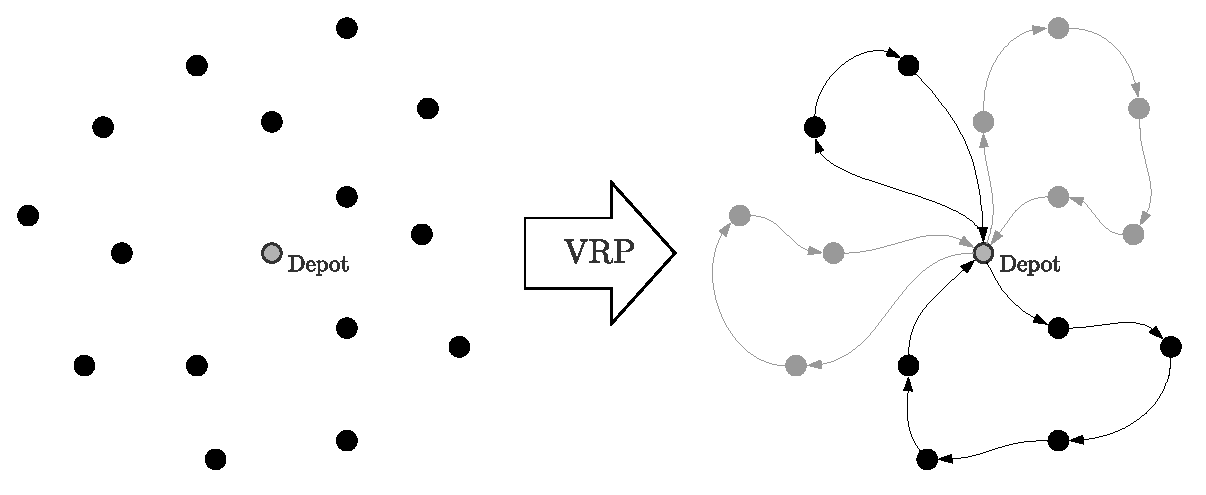
\includegraphics[width=0.8\textwidth]{figures/illustration.pdf}
		\caption[An intuitive view of the VRP instance and an example solution.]{An intuitive view of the VRP instance (left) and an example solution for four vehicles (right).}
		\label{fig:illustration}
	\end{figure}

In other words, the problem is concerned with finding the optimal routes to be followed by a fleet of vehicles to serve a set of customers \cite{golden2008the}. To better illustrate the problem, figure \ref{fig:illustration} shows an intuitive view of a VRP instance along with its example solution for four vehicles.

% Generally, in the VRP, the customers to be visited are modelled over graph nodes, whereas the problems where the requests are dispersed along the arcs are called \emph{arc routing problems} (ARP) \cite{corberan2014arc}.

The vehicle routing problem is one of the most studied problems in combinatorial optimization due to its relevance in industry \cite{golden2008the}. It belongs to the field of operations research applied to transportation problems. Figure \ref{fig:vrp-classes} shows the classification of VRP within operations research and puts in context the family of pickup and delivery problems that will be introduced later, and which is eminently important for this work.

	\begin{figure}[!ht]
		\centering
		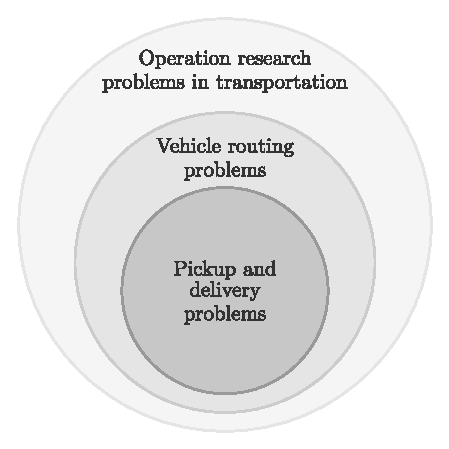
\includegraphics[width=0.6\textwidth]{figures/vrp-classes.pdf}
		\caption[The taxonomy of VRP and PDP within transportation-related operations research.]{VRP is one of many problems studied within transportation-related operations research. Pickup and delivery problems are a subclass of vehicle routing problems. The class of operations research contains many other problems apart from VRP, adopted from Ropke (2005)~\cite[p.~4~(modified)]{ropke-2005-phd}.}
		\label{fig:vrp-classes}
	\end{figure}

Numerous real-world applications have demonstrated the significance of computer-generated solutions of VRP in terms of global transportation costs \cite{toth2015vrp}. The success of optimization techniques can be attributed not only to the increasing computer power but also to recent research breakthroughs, the development of new mathematical models and to newly adopted approaches that leverage machine learning \cite{toth2015vrp, Falkner2020}. 

The VRP was first introduced in 1959 by Dantzig and Ramser \cite{1959} who came with the first mathematical model and an algorithmic approach using a simple matching-based heuristic. Since then, more than 80 years have passed and hundreds of models and algorithms have been proposed for different families of VRP as a result of a large variety of practical applications \cite{toth2015vrp}. This tendency has been enlarged by the burst of consumer delivery in the beginning of the century \cite{Falkner2020}. To show an example, the American logistics company UPS delivered around 11.5 million packages in 1993, compared to around 6.3 billion in 2020\footnote{\url{https://stories.ups.com/upsstories/us/en/about-us/global-presence/corporate-facts.html}} which counts for 24.7 million per single day.

Many variants of VRP have emerged over the years and the literature shows a clear trend towards the study of more complex variants to lower the gap between academic research and real-world applications. These problems imply constraints on various features the route must satisfy, such as vehicle capacity, pickup and drop-off times, or delivery sequence of operations. These classes of routing problems are often called \emph{rich VRPs} \cite{Mor2020}. These include \emph{capacitated VRP} (CVRP), in which each vehicle has predefined finite capacity that cannot be exceeded; the \emph{VRP with time windows} (VRPTW), where customers have to be served in predefined time intervals; the \emph{pickup and delivery problem} (PDP), where the goods (or people) to be transported have to be picked up at certain vertices as opposed to the depot; or the \emph{heterogenous fleet VRP} (HFVRP), in which vehicles may have different features, such as different capacities or can deliver only certain type of goods. Routing problems that involve transportation of people are referred to as \emph{dial-a-ride problem} (DARP) (or \emph{dial-a-flight problem} (DAFP) for air transportation) \cite{golden2008the, PILLAC20131}. These prevailing variants are detailed in the following sections and their taxonomy is clearly shown in figure \ref{fig:vrp-variants}. It is important to mention that these variants make just a fraction of the variants studied in the literature. Moreover, the distinction between the following variants of VRP is not always sharp and many combinations have been derived to more precisely represent real-world problems \cite{golden2008the, toth2015vrp, 2007-cordeau, cordeau-2007-7}.

	\begin{figure}[!ht]
		\centering
		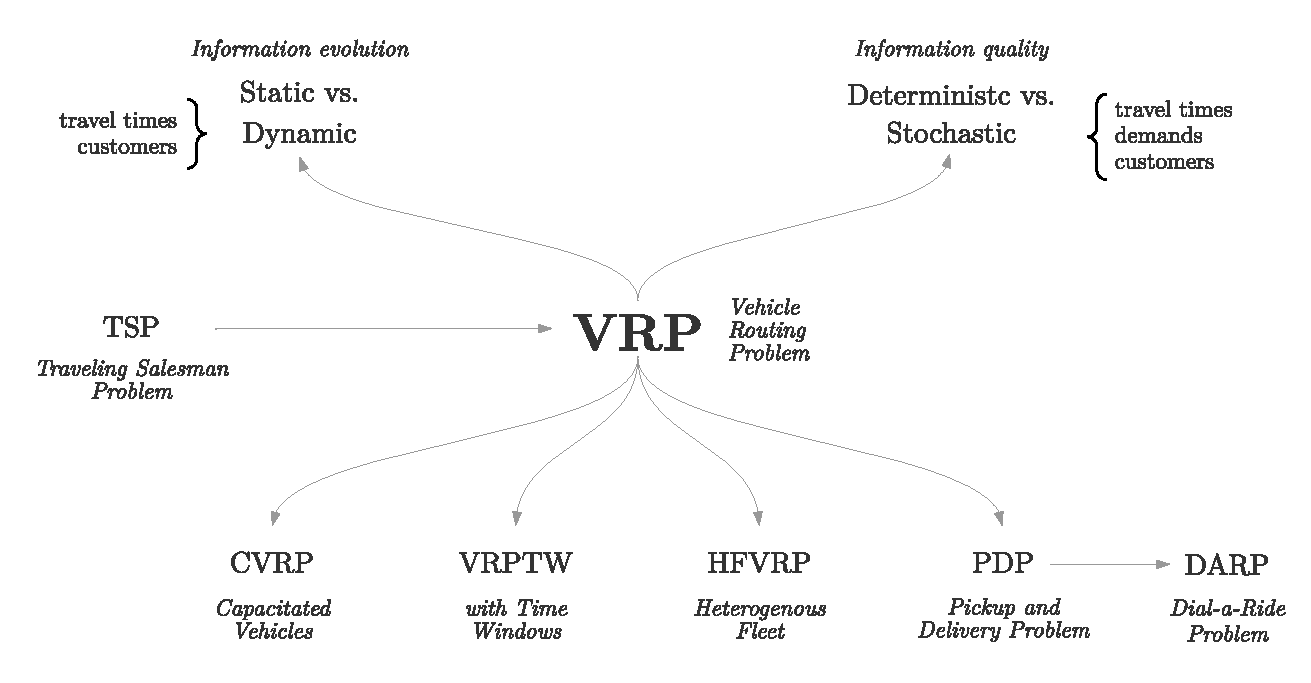
\includegraphics[width=1\textwidth]{figures/vrp-variants.pdf}
		\caption[Taxonomy of the VRP.]{Taxonomy of the VRP - the figure shows the prevailing variants of the VRP and common examples of static and dynamic elements, adopted from Bono (2020)~\cite[p.~26~(modified)]{Bono2020}.}
		\label{fig:vrp-variants}
	\end{figure}

\subsection{Capacitated Vehicle Routing Problem (CVRP)}

This variant of routing problems is the most studied in the literature, although it is mostly of academic relevance \cite{toth2015vrp}. In CVRP the requests correspond to the transportation of goods from a single depot to a set of customers. Each customer has a \emph{demand}, which is the amount to be delivered. The vehicle fleet is typically \emph{homogenous}, meaning that all vehicles have the same finite capacity and the same operational cost. Each vehicle starts at the depot, serves a disjunct set of customers, and returns to the depot \cite{toth2015vrp, cvrp-2019}.

\subsection{Vehicle Routing Problem with Time Windows (VRPTW)}

VRPTW is an extension of CVRP where the service at each customer location must occur within predefined time intervals, referred to as \emph{time windows}. There are two types of time windows commonly distinguished: soft and hard. Soft time windows can be violated carrying a penalty cost. In case of hard time windows, a driver must not arrive outside of the interval. The driver may arrive to the customer before the time window, however, the customer cannot be serviced until the time window starts. Arriving after the end of the time window is prohibited. Time windows can also be one-sided, i.e., defined as the earliest or the latest time of delivery \cite{wrptw, toth2015vrp, 2007-cordeau}.

\subsection{Heterogenous Fleet Vehicle Routing Problem (HFVRP)}

In this variant, vehicles are characterized by different features, such as different capacities, operational costs, or can only deliver a certain type of goods \cite{golden2008vrp, hvrp-2016, hvrp-2019}. There are two main branches of HFVRP regarding the obtainable fleet. In the \emph{unlimited} HFVRP, known as \emph{fleet size and mix VRP} (FSMVRP), the problem is to find the best fleet composition and routes, assuming that there is an unlimited number of vehicles of each type. In opposition, in the \emph{limited} HFVRP, known as \emph{heterogeneous VRP} (HVRP), the task is to find the optimal routes for the available fixed vehicle fleet \cite{hvrp-2019}. The cost of the solution usually depends on either the total distance traveled by all vehicles or the total enroute time. This problem is sometimes augmented by introducing time window constraints, making the HFVRP with time windows (HFVRPTW) \cite{hvrp-2016}.

In recent years, a relatively new variant related to HFVRP has emerged, called the \emph{green vehicle routing problem} (Green-VRP). The aim of Green-VRP is to minimize fuel consumption and to maximize the use of alternative fuel vehicles, such as electric vehicles, to reduce the impact on the environment. Usually, a heterogenous fleet of both classic and alternative fuel vehicles is considered during the planning process \cite{Asghari2021}.

\subsection{Pickup and Delivery Problem (PDP)}

Three known types of pickup and delivery problems are generally distinguished in the literature \cite{cordeau-2007-7, toth2015vrp}. First, the \emph{single-commodity} PDP, where a single type of good is either picked up or dropped-off at each of the customer location. An example of this problem might be transporting money from bank branch offices via an armored vehicle. Second, the \emph{two-commodity} PDP, in which two types of goods are being transported and each customer location may be used for both pickup and drop-off. This problem might occur, for example, in distribution of beverages, where the driver simultaneously delivers full bottles to the customer and collects the empty ones. A variant of the two-commodity PDP is a VRP with backhauls, where a pickup is only allowed when the vehicle is completely empty \cite{wrptw}. Finally, the \emph{n-commodity} PDP is where each type of good is associated with a single pickup location and a single drop-off location. A typical example of this problem can be a food delivery service \cite{cordeau-2007-7, 8541149, hvrp-2020}. In the literature, this problem is often referred to as \emph{vehicle routing problem with pickup and delivery} (VRPPD) \cite{cordeau-2007-7}.

From the implementation perspective, PDP setting introduces a new set of constraints. First, the constraints for the routes, such that the pickup and drop-off must be taken care of by the same vehicle. Second, the precedence constraint, i.e., the pickup happens before the drop-off \cite{Bono2020}.

A typical extension of PDP emanating from real-life usecases is the PDP with time windows (PDPTW). In this case, each pickup (drop-off) node is associated with a time interval, in which the driver can perform the pickup (drop-off) \cite{wrptw}.

\subsection{Dial-a-Ride Problem (DARP)}

The PDP also covers problems associated with people transportation. The major difference between transporting goods and people is the incorporation of customer satisfaction requirements. One of those problems is the so-called \emph{dial-a-ride problem} (DARP). This demand-responsive service is usually provided by a public authority to serve physically impaired people and elderly who may have difficulty using regular transport options \cite{toth2015vrp}. Unlike taxi and public transport services, passengers may share the ride with other passengers and, as a result, may deviate from the direct path from the pickup point to their destination \cite{darp-survey}. Some DARPs operate on a heterogenous fleet of vehicles, where different vehicles satisfy the different needs of physically impaired persons, for example, by being wheelchair accessible, some allow transfers from one vehicle to another \cite{belhaiza-2019, darp-survey}. The DARP implies that a set of customers make a request, which consists of origin and destination locations and imposes time window constraints for both pickup and drop-off. Additionally, customer inconvenience constraints are typically inflicted, such as maximum enroute time or maximum vehicle capacity \cite{toth2015vrp, belhaiza-2019}. There are three objectives of DARP that are often conflicting: maximizing the number of requests the fleet can serve, minimizing the overall operational cost, and minimizing customer inconvenience. A ratio between these objectives is sometimes achieved by first maximizing the number of requests that can be served by the available fleet of vehicles, and then minimizing the operational cost while acknowledging the inconvenience constraints \cite{cordeau-2007-7}.

Other people transportation problems related to DARP include \emph{dial-a-flight Problem} (DAFP) that concerns with air transportation \cite{PILLAC20131}, car pooling problem, which consists of finding groups of employees to share a car to work \cite{toth2015vrp}, Uber Pool service of an American company Uber \footnote{\url{https://www.uber.com/}} that combines taxi service with car pooling \cite{uber-pool}, or the \emph{school bus routing problem} (SBRP), where children in rural areas are picked up from the bus stop close to their homes and transported to their schools.


\subsection{Evolution and Quality of Information} \label{sec:evolution}

In contrast to the classical definition of VRP, real-world use cases often involve two important dimensions. The first one is \emph{evolution}, i.e., whether decisions are made a priori (referred to as \emph{static}) or the information changes in response to new information during the planning process, for instance, when new requests arrive or number of drivers changes (referred to as \emph{dynamic}). Second aspect is the \emph{quality of information}, i.e., whether the information is known with certainty before the start of planning (referred to as \emph{deterministic}) or there exists some amount of uncertainty when decisions are made (referred to as \emph{stochastic}). This categorization applies to VRP as well as DARP. \cite{PILLAC20131, darp-survey}

	\begin{figure}[!ht]
		\centering
		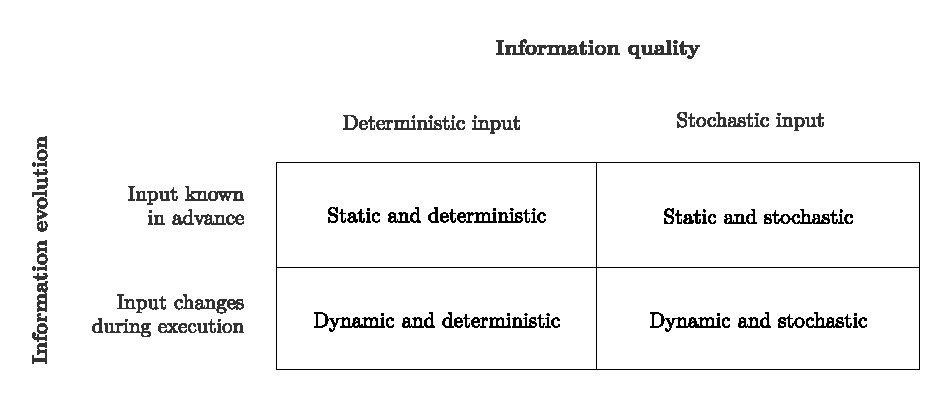
\includegraphics[width=0.9\textwidth]{figures/static-stochastic-table.pdf}
		\caption[Taxonomy of vehicle routing problems by information evolution and quality.]{Taxonomy of vehicle routing problems by information evolution and quality, adopted from Pillac et al. (2013)~\cite[p.~2~(modified)]{PILLAC20131}.}
		\label{fig:static-stochastic-table}
	\end{figure}

Based on these dimensions, four categories of routing problems are identified and are shown in figure \ref{fig:static-stochastic-table}. In \emph{static and deterministic} problem, all information is known before the decisions are made and does not change during the execution of planning. It is sometimes referred to as \emph{clasical} problem \cite{PILLAC20131}. \emph{Static and stochastic} problems are the ones where some information is unknown or uncertain at the time of decision, but information about the uncertainty may be known, i.e., in the form of an available range or probability distribution. In addition, routes are planned a priori and only slight changes are allowed during the execution, for example, adding a new node at the end of the plan or skipping a customer. These types of problems do not require any additional technological support. Most of the research in this field is focused on stochastic customers, stochastic time windows, and stochastic demands \cite{GENDREAU19963, 2007-cordeau, stoch-demands}.

\emph{Dynamic and deterministic} problems work with some part of the input that is unknown and revealed dynamically during the execution of planning. Thus, the routes for the drivers need to be constantly updated, which requires additional technological support for providing additional information to the planner, such as the location of the drivers using their mobile phones with GPS \cite{2007-cordeau, online-routing-2007}. Some authors also call these problems \emph{real-time} or \emph{online} \cite{online-routing-2007}. \emph{Dynamic and stochastic} problems are similar to the previous type, but additionally, stochastic knowledge about the dynamically revealed information is available.



\section{Solution Methods}

The approaches to solve vehicle routing problems are generally divided into two categories: exact and heuristic. The exact methods guarantee to find the optimal solution when sufficient resources are provided. However, until now, only small instances of VRP problems involving only up to tens of customers can be solved optimally due to high computational complexity \cite{toth2015vrp, Peng2020}. Indeed, VRP belongs to the class of NP-hard problems \cite{time-complexity-vrp}. Moreover, according to Savelsbergh (1985) \cite{Savelsbergh1985}, even finding a feasible solution for the VRPTW is itself an NP-complete problem. Nonetheless, some amply constrained problems with reasonable-sized instances can be solved to optimality via mathematical programming techniques \cite{2007-cordeau}, which are covered in section~\ref{sec:exact-methods}.

In real-life problems, exact methods are oftentimes insufficient as large instances need to be solved in a relatively short time. Therefore, heuristic approaches are required to tackle real-world problems. With the trade-off between the computation time and optimality, heuristic algorithms are able to find solutions of relatively good quality within acceptable computational time even for large instances \cite{Peng2020}. In addition, heuristic algorithms offer a decent amount of flexibility which allows to target different problem settings that vary in constraints and objectives \cite{toth2015vrp}. However, heuristic algorithms lack the theoretical guarantee regarding the quality of produced solution. Observations about solution quality can only be made empirically based on experiments \cite{ropke-2005-phd, Peng2020}.

A class of heuristic algorithms that has gained attraction over the last years is \emph{metaheuristics}. They provide a general framework for heuristics applicable to many problem variants and they often generate solutions of very high quality \cite{ropke-2005-phd}. In fact, metaheuristics are capable of yielding solutions within seconds whose values lie within one percent from the best known values \cite{toth2015vrp}. Heuristic algorithms are further described in section \ref{sec:heuristics}.

Another special class of heuristics that should be mentioned are \emph{approximation algorithms}. These methods provide both a solution and an error guarantee. For instance, they could guarantee that the obtained solution is at most $k$ times worse than the best obtainable solution \cite{vazirani2001approximation}.

% However, approximation algorithms are not the focus of this work and will not be covered in more detail.

The following sections provide an overview of both exact and heuristic methods for solving the VRP. More emphasis is being put on metaheuristic approaches as they are currently the state-of-the-art solution for most real-world VRP problems \cite{toth2015vrp}.

\subsection{Exact Methods} \label{sec:exact-methods}

For many real-world problems, the solution space is so large that even if we had a computer that could evaluate the cost of a trillion solutions per second, and we had started it right after the big bang, around 14 billion years ago, it would not have evaluated all feasible solutions by today. Therefore, exact algorithms need to use other methods rather than simple enumeration \cite{ropke-2005-phd}. This section lists a few most popular exact methods. For a detailed description and an extensive survey, we refer the readers to Toth and Paolo (2015) \cite{toth2015vrp} and Ho at al. (2018) \cite{darp-survey}.

The CVRP is the oldest and the most basic variant of the VRP, hence the first exact methods were developed mostly for the CVRP and later extended to be used with other VRP variants. The CVRP is an extension of the known \emph{travelling salesman problem} (TSP), where the task is to find a Hamiltonian circuit with minimum cost while visiting each node exactly once \cite{toth2015vrp}. The TSP was first formulated in 1930, around 30 years earlier than the VRP \cite{tspsurvey, 1959}. Therefore, the foundation of many exact algorithms for the CVRP builds on the thorough work done for the exact solution of the TSP \cite{toth2015vrp}. However, as it turns out, the CVRP is significantly harder to solve in practice compared to the TSP. The best exact methods for the CVRP are rarely able to solve instances with over a hundred customers, whereas the TSP instances with thousands of nodes are now routinely solved to optimality \cite{2007-cordeau}.

Exact methods directly address the problem using integer linear programming. The objective is to find a binary assignment for decision variables, modelling connections between vehicles and nodes, while minimizing the objective value \cite{Bono2020}. The early methods to solve the CVRP were mainly direct tree search algorithms based on branch-and-bound (B\&B) \cite{toth2015vrp}. Algorithm \ref{alg:bab} shows a main loop of branch-and-bound.

The computational complexity of the B\&B can be exponential in the worst case \cite{darp-survey}, thus some relaxations need to be employed to speedup the search. The combinatorial relaxations used in the branch-and-bound algorithms were adopted from what was earlier proposed for the TSP \cite{tspalg} and later extended by better relaxation techniques based on Lagrangian relaxations and the additive approach. These methods were able to solve instances with lower tens of customers to optimality \cite{toth2015vrp}. Later, branch-and-cut algorithms exploited cutting planes to tighten the linear programming relaxations, which led to a higher chance of finding integer solutions, and provided stronger bounds for optimality verification. In contrast, branch-and-price algorithms focused on column generation rather than generating cuts, which allowed to solve larger mixed-integer programs while still guaranteeing the convergence to global optimum \cite{toth2015vrp, darp-survey}. Current best algorithms for the CVRP belong to the branch-and-price-and-cut family, which combines cuts and column generation, and are much more effective than each of those techniques alone \cite{Fukasawa2006}.


\begin{algorithm}[!ht]
\SetAlgoLined
 currentBest, upperBound $\leftarrow$ FindInitialSolution(problem)\;
 add problem to queue\;
 \While{queue is not empty}{
  problem $\leftarrow$ pop item from queue\;
  \For{subProblem in branch}{
    \If{CanSolve(subProblem)}{
     candidate, cost $\leftarrow$ Solve(subProblem)\;
     \If{cost $\leq$ upperBound}{
      currentBest, upperBound $\leftarrow$ candidate, cost\;
     }
    }
    \ElseIf{LowerBound(subProblem) $\leq$ upperBound} {
      add subProblem to queue\;
    }
  }
 }
 \caption{Branch-and-Bound, adopted from Bono (2020)~\cite[p.~34~(modified)]{Bono2020}.}
 \label{alg:bab}
\end{algorithm}

Branch-and-price is largely used for solving a variety of routing problems and is not constrained to only the CVRP. For the VRPTW, this approach was first used by Desrochers, Desrosiers, and Solomon (1992) \cite{Desrochers1992}. The branch-and-price-and-cut algorithm was also later applied to VRPTW by Kohl et al. (1999) \cite{Kohl1999}.

Similarly, for the pickup and delivery problems, Lu and Dessouky (2004) \cite{branchAndCut} and later Ropke et al. (2007) \cite{branchAndCut2} have used the branch-and-cut algorithms for the PDPTW. Their approach was able to solve instances of up to 75 customers to optimality. The branch-and-cut-and-price algorithm by Ropke et al. (2009) \cite{branchCutPrice} was able to solve some highly constrained instances of PDPTW of up to 500 customers. In the DARP setting, most of the exact methods are also built upon the concept of branch-and-bound \cite{darp-survey}. For multiple vehicles, methods based on branch-and-price seem to be the most promising in the current state of the art. Still, most PDP instances remain much harder to solve than the same-size instances of classical VRP. This is predominantly caused by the precedence constraints, which generally lead to poor linear programming relaxations \cite{toth2015vrp}.

The main advantage of using the exact methods is that the optimality of the solution is guaranteed. This is particularly important for static problems. Therefore, the majority of the research in exact algorithms focuses on static and deterministic problems. Computational times of several hours are acceptable for problems, where the information is provided in advance and no changes are expected. Even if the optimal solution cannot be retrieved by the exact algorithm, the planner is able to measure the optimality gap, aka how far the solution can be from the optimum \cite{darp-survey}.


\subsection{Heuristic Methods} \label{sec:heuristics}

When problems are not manageable by exact methods, for instance, due to unacceptable computational time or memory issues, heuristics are essential to provide high-quality solutions \cite{darp-survey}. The field of VRP heuristics is so rich nowadays that it would be an unimaginable task to describe or even list all of them in this section. Instead, we summarize the most prevailing methods that are still being actively used and present some new and promising techniques.

The progression of heuristic approaches for VRP in the last decade has been primarily in the context of metaheuristics. What best describes this progression is the hybridization of both concepts and scope. First, there has been an emergence of new heuristics that combine several concepts in terms of search principles that have been initially developed individually, such as genetic algorithms, tabu search, large neighborhood search, or simulated annealing. In addition, other strategies and techniques have found their place in the most popular methods. These include exotic large neighborhoods, exact mathematical techniques, decomposition, and cooperation schemes, to name a few. Second, the hybridization of scope in heuristics means that they offer a decent amount of flexibility which allows to target different problem variants with various constraints and objectives without any extensive structural changes \cite{toth2015vrp}.

The following two sections summarize some relevant results regarding constructive heuristics and metaheuristics. We also take a brief look at the latest advancements in machine learning methods for VRP.

\customsubsubsection{Constructive Heuristics}

Constructive heuristics are frequently utilized to quickly create an initial feasible solution. Although metaheuristics are more effective, constructive heuristics are employed in various dynamic problems that require a feasible solution within milliseconds \cite{Markovic2015, Wong2014}, or to evaluate various operational policies \cite{Wong2014}. In many cases, solutions obtained via constructive heuristics are used to provide an initial solution for more complex methods \cite{Masmoudi2016, Braekers2014}. However, many metaheuristics are so robust that they can be initialized with any random solution, which does not even need to be feasible, and still produce high-quality results \cite{toth2015vrp}.

Most constructive heuristics are inspired from the greedy insertion heuristic introduced by Jaw et al. (1986) \cite{Jaw1986}, who was the first to adapt the traditional insertion algorithm to DARP with time windows and multiple vehicles. The algorithm selects the requests sorted by the earliest pickup time and inserts the request into the cheapest feasible position in the existing routes. Alternatively, it adds a new vehicle if no feasible position is found.

Lu and Dessouky (2006) \cite{insertionHeuristics} proposed an insertion-based heuristic for the PDPTW, which regarded the deviations from time windows and an increase in travel time. The results show that the heuristic outperforms several decent methods on standard benchmarking problems. A similar approach was taken by Fielder et al. (2018) \cite{fiedler} in a dial-a-ride setting.

\customsubsubsection{Metaheuristics}

Metaheuristics for the VRP can be loosely classified into two categories: local search methods and population-based methods. However, the frontiers between these methods have become increasingly fuzzy in recent years and many hybrid methods have emerged. They will also be discussed in this section.

Local search algorithms start from an initial solution $x_0$ and at each iteration $t$, they move from the current solution $x_t$ to another solution $x_{t+1}$ in its neighborhood $N(x_t)$. The neighbors are retrieved by applying operators, which make minor modifications of the original solution. If any neighbor yields a better performance, i.e., the cost $c(x_{t+1})$ is lower than $c(x_t)$, it becomes the new candidate solution. However, local search algorithms usually allow worsening of the solutions, such that the cost $c(x_{t+1})$ does not always have to be lower than $c(x_t)$, to better explore the solution space and escape the local optimum. As a result, certain mechanisms must be put in place to avoid cycling \cite{Bono2020, toth2015vrp}. Algorithm \ref{alg:local-search} shows a common main loop of local search algorithms.

\begin{algorithm}[!ht]
\SetAlgoLined
 candidate $\leftarrow$ FindInitialSolution()\;
 best $\leftarrow$ candidate\;
 \While{stopping criterion is not met}{
    \If{IsValid(candidate) and Cost(candidate) $<$ Cost(best) }{
     best $\leftarrow$ candidate\;
    }
    neighbor $\leftarrow$ FindBestNeighbor(candidate)\;
    \If{Cost(neighbor) $<$ Cost(candidate) or AllowWorse(neighbor)} {
      candidate $\leftarrow$ neighbor\;
    }
 }
 \caption{Local Search, adopted from Bono (2020)~\cite[p.~36~(modified)]{Bono2020}.}
 \label{alg:local-search}
\end{algorithm}

\customparagraph{Tabu Search}

One of the local search algorithms is \emph{tabu search}. It moves from a solution $x_t$ to the best non-tabu solution $x_{t+1}$ in its neighborhood $N(x_t)$. To avoid cycling, it keeps a list of previous candidate solutions that are declared \emph{tabu}, or forbidden, to the completion of the algorithm, or for a certain number of iterations \cite{toth2015vrp}.

Tens of different implementations of tabu search have been proposed over the years. One of the first metaheuristics for PDPTW was an algorithm proposed by Nanry and Barnes (2000) \cite{nanryBarnes}. They developed the tabu search with three operators: moving a pickup-drop pair into another plan, switching two pickup-drop pairs between plans and moving individual nodes within the plan. Cordeau and Laporte (2003) \cite{Cordeau2003} were among the first to use the tabu search for the DARP with satisfactory results. Moreover, Zachariadis and Kiranoudis (2010) \cite{Zachariadis2010} showed that tabu search can perform very well even on large-scale instances.

\customparagraph{Simulated Annealing}

\emph{Simulated annealing}, another well-known local search operator uses a technique inspired by the physical annealing process. The solution $x_{t+1}$ is usually randomly selected from the neighborhood $N(x_t)$. To avoid being stuck in a local optimum, worse or nonimproving solutions are accepted with a given probability \cite{Bono2020}. One known implementation of this algorithm for the VRP is that of Osman (1993) \cite{Osman1993}.

One of the recent studies conducted by Braekers et al. (2014) \cite{Braekers2014} proposed a highly effective deterministic variant of simulated annealing, named \emph{deterministic annealing}. In this study, nonimproving solutions are accepted while the deterioration of the objective value is lower than a deterministic threshold. Braekers et al. used more complex operators and, in addition, a restart strategy to escape unattractive regions of the search space.

\customparagraph{Variable Neighborhood Search}

Both the tabu search and simulated annealing work well as standalone algorithms, but are widely used in combination with local search heuristics, such as \emph{variable neighborhood search} \cite{Gendreau2001, Schneider2014}. This algorithm was first proposed by Mladenovi{\' c} and Hansen (1997) \cite{Mladenovic1997}. It works with several neighborhoods ($N_1,\ldots,N_p$) that are systematically changed in the descent and preturbation phases of the local search. The algorithm starts from an initial solution $x_0$ and iteratively applies these neighborhoods until no improvement is achievable. After the last applied neighborhood, the cycle restarts. The algorithm usually finishes after a defined number of cycles or, as introduced by Li and Lim (2003) \cite{liLim}, when the solution is no longer improving.

Kytöjoki et al. (2007) \cite{KYTOJOKI2007} were among the first who successfully applied variable neighborhood search to solve the VRP. Two years later, Parragh et al. (2009) \cite{Parragh2009} proposed a variable neighborhood search for the DARP. Thanks to the great results, more researchers have adapted the algorithm to other DARP usecases in recent years \cite{SCHILDE2011, SCHILDE2014, MUELAS2013, MUELAS2015, Detti2017}. Variable neighborhood search proved to be able to obtain high-quality solutions even for large-scale VRP instances of up to 20,000 customers \cite{toth2015vrp}.

\customparagraph{(Adaptive) Large Neighborhood Search}

One of the most successful metaheuristics for a wide variety of routing problems is \emph{large neighborhood search} \cite{Gschwind2016}, first introduced by Shaw (1997) \cite{Shaw1997}. At each iteration, part of the current solution is destroyed (e.g., $k$ requests are removed) by applying one or more removal operators and rebuilt again into a new complete solution using one or more insertion operators \cite{darp-survey}. The modifications of solutions are commonly bigger than those of previously described heuristics. In an adaptive extension of this algorithm, called \emph{adaptive large neighborhood search}, the removal and insertion operators are selected based on their past performance during the search, usually by employing a roulette wheel selection process with an adaptive weight adjusting mechanism \cite{Azi2014, Gschwind2016, Masmoudi2020}.

Ropke and Pisinger (2006) \cite{Ropke2006} used the adaptive large neighborhood search heuristic to solve the PDP with time windows. Their algorithm used removal and insertion operators already existing in the literature, including the removal operator by Shaw (1997) \cite{Shaw1997}, and an acceptance criterion for new solutions known from simulated annealing. The algorithm by Ropke and Pisinger has proven to be powerful and has served as a building block for many further studies in complicated routing problems, particularly PDP and DARP \cite{Gschwind2016, Braekers2016, Masmoudi2016, Belhaiza2017, Drexl2018, Belhaiza2019, Masmoudi2020, Wang2020, Cauchi2020, Malheiros2021}. Gschwind and Drexl (2016) \cite{Gschwind2016} adopted the algorithm from Ropke and Pisinger and added three more removal operators. They also demonstrated how to test a new solution for feasibility in an amortized constant time. Their version of the adaptive large neighborhood search produced better solutions on standard DARP instances compared to the vast majority of other algorithms, except for the hybrid genetic algorithm by Masmoudi et al. (2017) \cite{Masmoudi2017}.

\vspace{0.5cm}

The other well-known category of metaheuristics are population-based methods, which are inspired by natural processes, such as the evolution of species or the behavior of insects. All successful population-based heuristics rely on local search methods to drive the search towards promising areas and to avoid local optima. As a result, the majority of population-based algorithms are naturally hybrid \cite{toth2015vrp}.

\customparagraph{Ant Colony Optimization}

This metaheuristic has also proven practical for many routing problems. It is inspired by the pheromone mechanism used by ants for coordination. Each ant simulates a solution by traversing the graph along its edges and accumulates pheromons along the edges it traversed. In each iteration, the ants select the edges with a probability proportional to the pheromon value. The pheromon evaporates after a given number of iterations, so the most promising edges remain at the end \cite{Bono2020, Solnon2010}. The algorithm by Reimann et al. (2004) \cite{Reimann2004} was one of the most successful.

Ant colony optimization algorithm is particularly interesting in dynamic and stochastic settings. When new information is received, such as a new request arrives, or some delays occur, the algorithm uses the pheromone trails from previous iterations. This relies on the assumption that the new information does not disrupt the current solution too much and that some patterns can still be exploited \cite{Schyns2015, Bono2020}.

\customparagraph{Genetic Algorithms}

\emph{Genetic algorithms} are population-based methods that are inspired by the evolution of species. These algorithms usually work with not a single solution, but rather a population of solutions, called \emph{individuals}. At each iteration, the individuals with better fitness are selected with higher probability to be parents. New individuals are created by applying the crossover and mutation operators to the parents and added to the population, while some other individuals are replaced \cite{Bono2020, darp-survey}.

The first successful application of genetic algorithms to solve the VRP is that of Prins (2004) \cite{Prins2004}. Prins combined the genetic operators, selection and crossover with a local search method to replace the classic random mutation operator. Other researchers successfully applied genetic algorithms for numerous VRP variants, for example, Masmoudi et al. (2017) \cite{Masmoudi2017} proposed a hybrid genetic algorithm to tackle the DARP with excellent results, even outperforming in terms of quality of solution, many large neighborhood search algorithms that are usually better performing on larger instances \cite{darp-survey}.

\customsubsubsection{Hybrid Algorithms}

Combining metaheuristics with other metaheuristics or exact methods is a growing trend that has proven successful. Indeed, many state-of-the-art algorithms for combinatorial optimization problems are hybrid algorithms.

In the literature, hybrids of metaheuristics are the most prevalent \cite{darp-survey}. They usually come in two forms. First, each metaheuristic is executed sequentially, for example, in a study by Parragh et al. (2009) \cite{Parragh2009}, where several algorithms are applied to the best solutions obtained from the previous algorithms. The other option is that one metaheuristic is executed in another metaheuristic. A popular approach is to embed local search methods into population-based heuristics, which takes advantage of combining the exploration ability of population-based heuristics with the exploitation ability of local search methods. Examples of this approach are the studies by Masmoudi et al. (2016 and 2017) \cite{Masmoudi2016, Masmoudi2017}.

Hybrids of metaheuristics with exact methods are also employed. They are obtained by either embedding a metaheuristic to the mathematical or constraint programming approach or vice versa. An example could be a research conducted by Parragh and Schmid (2013) \cite{Parragh2013}. They combined a column generation approach with a variable neighborhood search. To improve the obtained solutions, a large neighborhood search was employed. Another example could be the study by Gschwind and Drexl (2016) \cite{Gschwind2016} in which dynamic programming
is used within a large neighborhood search.

\customsubsubsection{Leveraging Machine Learning} \label{sec:machine-learning}

Designing a good heuristic algorithm is difficult as it requires expert knowledge of the problem and often involves the incorporation of custom features or constraints. Several alternative approaches have been proposed that use neural networks to learn heuristics directly from data. The performance of these heuristics has been improving in recent years, however, pure machine learning approaches are still usually outperformed by classical optimization methods \cite{Peng2020, Hottung2019}.

One of the early research in this field was by Potvin et al. (1996) \cite{Potvin1996}, who used a competitive neural network model and a genetic algorithm to improve a parallel insertion heuristic introduced by Potvin and Rousseau (1993) \cite{POTVIN1993331} for the VRPTW.

Since then, machine learning algorithms have been significantly improved and seem to be the focus of many researchers. Recently, Kool et al. (2019) \cite{Kool2019} has proposed a new attention model for learning heuristics for optimization problems and presented a learning mechanism based on reinforce. This model has been one of the building blocks of a research conducted by Peng et al. (2020) \cite{Peng2020} who presented a dynamic attention model with dynamic encoder-decoder architecture, which, based on the results, outperforms the attention model presented by Kool et al.

Still, the prevailing problem with machine learning approaches is that they lack flexibility in terms of different features, constraints, and objectives. As in response to this problem, in the last two years, several studies have emerged that have made a notable leap in this area \cite{Nazari2018, Hottung2019, Falkner2020, Li2021}.

The capacity constraints were introduced in a recent study by Nazari et al. (2018) \cite{Nazari2018}, who used reinforcement learning to solve the CVRP. Their approach outperforms Google's OR-Tools\footnote{See section \ref{solvers} for details about OR-Tools.} on medium-sized instances within comparable computational time and has the potential to be used on other VRP variants or even other combinatorial optimization problems. Furthermore, Hottung and Tierney \cite{Hottung2019} proposed a large neighborhood search combined with a deep neural network with an attention mechanism to solve CVRP. They were able to outperform large neighborhood search methods based on classical optimization techniques on instances of around 300 customers. Recently, time windows were successfully tackled by Falkner and Schmidt-Thieme (2020) \cite{Falkner2020}.

Some other features have been successfully incorporated into machine learning models. Falkner and Schmidt-Thieme (2020) \cite{Falkner2020} presented an algorithm that successfully solves VRP with time windows. Similarly, Li et al. (2021) \cite{Li2021} showed how to solve PDP via deep reinforcement learning.

All mentioned works use generated instances in a two-dimensional space where the distances between nodes are measured by Euclidian distance. To the best of our knowledge, no study has used real distances and durations between the nodes, as well as more sophisticated features like different service times at each location, different depots, or already picked up deliveries in a dynamic setting. Therefore, more research has to be done to successfully deploy those techniques into practice.

\subsection{Methods for Solving Dynamic Problems} \label{sec:dynamic}

This section briefly focuses on the recent research of dynamic problems defined in section \ref{sec:evolution}. In this context, heuristic approaches are prevalent for two reasons. First, the majority of real-world dynamic problems are too complex for exact algorithms to provide a solution in a reasonable time \cite{Bono2020}. Second, information is revealed over time and the complete instance is only known at the end of the planning horizon. As a consequence, even though the exact methods can provide an optimal solution for a current instance, they cannot guarantee that the solution remains optimal after new information is revealed \cite{PILLAC20131}.

Approaches for dynamic VRPs are based on either \emph{periodic reoptimization} or \emph{continuous reoptimization}. Periodic reoptimization approaches start with the initial set of routes and trigger the replanning procedure in response to information changes or at given time intervals. In each replanning procedure, the optimization algorithm works on the static problem. The main disadvantage of this method is that the optimization must be executed on each change, which is time-consuming, and sometimes impractical, given the nature of dynamic problems \cite{PILLAC20131, darp-survey}.

Approaches based on continuous reoptimization maintain information about good solutions in an adaptive memory. When the known information is updated, a decision procedure exploits the gathered memory using lookup strategies, such as Monte-Carlo trajectory sampling \cite{Bono2020}, to produce a new solution. These approaches usually require more complex implementation, however they maximize the computational capacity and have a net advantage compared to the previous category \cite{PILLAC20131, Bono2020}. 

\subsection{Available Solvers} \label{solvers}

There is a number of open-source and commercial solvers available for the most prevailing variants of the VRP.  Important questions that arise regarding solving real-world problems are regarding the quality of the produced solution, generality, flexibility, or speed. This section lists the most popular solvers and puts these questions into context.


A popular tool mainly in the industry is \emph{OR-Tools}\footnote{\url{https://developers.google.com/optimization}}, an open-source project by Google. It can be used to solve various combinatorial optimization problems and it provides wrappers for several languages, including Python, Java, C++, and C\#. In the context of VRP, OR-Tools supports many features, such as pickup and delivery, time windows, multiple depots, different start and end locations of drivers, capacity, skills, etc. In addition, Google provides developers with a rich documentation and an active community \cite{ortools, Karkula2020}.

There are 14 search strategies that can be selected for the VRP, including simulated annealing, tabu search, or greedy descent. Additionally, 13 different strategies to find an initial solution are available, such as \emph{parallel cheapest insertion}. The \emph{automatic} initial solution strategy lets the solver select the strategy automatically based on the problem variant \cite{ortools}.

The limitations of OR-Tools arise when larger instances need to be tackled. In some cases, changing the search options for the solver or a strategy for finding an initial solution can help, but generally the instances of rich VRPs, such as the PDPTW, are intractable for OR-Tools \cite{Karkula2020}.

Another commonly used open-source software for solving the VRP is \emph{Vehicle Routing Open-source Optimization Machine} (VROOM)\footnote{\url{https://github.com/VROOM-Project/vroom}}. It can find good solutions in small computing times and can scale for larger instances. Besides the common features like time windows and capacity, it supports some infrequent features, such as driver breaks and working hours. It is not only a VRP solver, but it bundles out-of-the-box integration with routing engines to produce cost matrices based on map data, which makes it easier to use in a real-world setting \cite{vroom}.

VROOM includes several heuristics for finding an initial solution that are selected automatically based on the specific use case. These include \emph{Christofides heuristics}, \emph{clustering heuristics}, or \emph{Solomon insertion heuristics}. The optimization algorithm behind VROOM is a local search procedure that uses 14 different exchange and reallocate operators \cite{Braysy2005, Karkula2020}.

Yet another open-source software that deserves attention is \emph{jsprit}\footnote{\url{https://github.com/graphhopper/jsprit}}, which is a Java based, open-source toolkit for solving TSP and VRP. Similarly to OR-Tools and VROOM, jsprit can solve problems with all classic features. Additionally, it allows to define additional constraints. It is well-documented and benchmarked on classic VRP instances \cite{jsprit}. The optimization mechanism behind jsprit is based on the large neighborhood search \cite{Karkula2020}.


\chapter{Problem Definition} \label{chapter:problem}
The literature review introduced the vehicle routing problem and presented the available solution methods. In this chapter, we demonstrate a real-world problem of route planning in food delivery and elaborate the constraints and objectives in detail.

The objective of this work is to come up with a suitable approach for the planning of food delivery. Food delivery may involve several categories, such as recurrent meal box delivery, grocery delivery, or delivery of ingredients. In this article, the term food delivery will be used to refer to online restaurant delivery, which is a courier service in which a restaurant or a third party logistics company delivers food to a customer. This food is typically fresh (hot or cold) and is intended to be eaten right away. Therefore, the food is picked up by the driver soon after it is prepared by the restaurant. The delivery orders are typically on demand, i.e., the customers expect their food to arrive in a short period of time after placing the order. These orders are placed via restaurant websites, a phone call, or a mobile application \cite{food-delivery2020}.

The prepared food is prone to damage if dropped, tilted, or kept for a longer duration. Therefore, technology must be involved in the process of food delivery. Food portions are usually packed in plastic or paper containers which are stored in thermal bags or boxes while being carried by the courier. In addition, to reduce the duration from cooking to delivery and, consequently, to ensure customer satisfaction, software tools and planning need to be engaged \cite{food-delivery2020}.

The costs associated with the delivery service are paid either by the customer, the restaurant, or are split between both parties. These costs include drivers' salaries, gas costs, vehicle amortization, or other transportation costs. The aim of the planning procedure is to minimize those costs and consequently, increase the revenue of the service. However, in the food delivery business, customer satisfaction is commonly the most important objective, because it results in customer retention, ultimately leading to a scalable and successful business.

From the VRP perspective, food delivery has its own specifics compared to other categories of logistics. The four most important ones with respect to route planning are:
\begin{description}
    \item[Dynamicity] New information is revealed during the day, such as the arrival of new orders, unexpected delays due to traffic, or changing the number of drivers. Therefore, high emphasis is placed on the speed of the selected algorithm, as the drivers need to react to changes as quickly as possible.
    \item[Short Time Windows] Customers expect their food to arrive shortly after they order it. In addition, ready-to-eat food has short lastingness and needs to be delivered as soon as possible to secure its quality.
    \item[Soft Time Window Constraints] The time windows for food delivery are generally soft, meaning they can be violated carrying a penalty cost. In addition, visiting a customer before the specified time window is usually preferred over being late, so the penalty is lower in that case.
    \item[Peak Times] Food delivery has peak times around lunchtime and dinnertime. With this, the number of required drivers need to change dynamically according to the time of the day.
\end{description}
    
\section{Formal Definition}
    
    It is clear that in the context of food delivery, each customer request consists of transporting goods (food) from one pickup location to one drop-off location. As there may be more restaurants preparing food, rather than a single depot, it is the case of \textit{pickup and delivery problem} (PDP). Since food delivery commonly involves multiple drivers and time window constraints, the ultimate generalization of this problem can be referred to as the \textit{pickup and delivery problem with time windows} (PDPTW). This variant also involves capacity constraints, i.e., how many food portions can each driver carry at any moment. In addition, one feature that is required for our use case is that the drivers can start at arbitrary locations rather than a single depot. An example of a single request is shown in figure \ref{fig:example-request}.
    
    \begin{figure}[!ht]
        \centering
        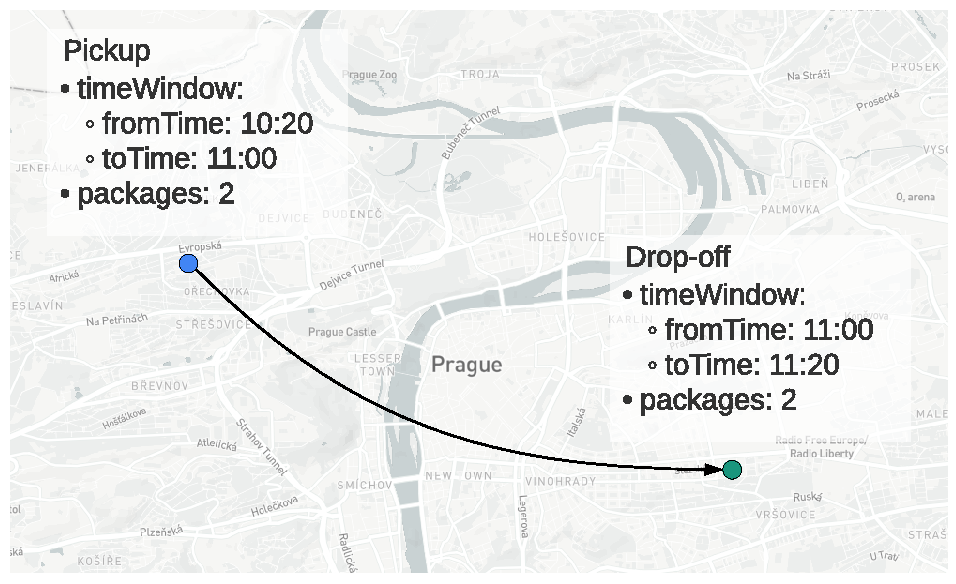
\includegraphics[width=0.8\textwidth]{figures/example-request.pdf}
        \caption{An example of a single request.}
        \label{fig:example-request}
    \end{figure}
    
    Using a similar notation to Cordeau (2006) \cite{cordeau}, let us define this problem formally:
    
    We are given a complete graph $G = (V,A)$, where $V$ is the set of nodes and $A = \{(i,j) : i,j \in V, i \neq j \}$ is the set of arcs. $V$ is further partitioned into three subsets $V = S \cup P \cup D$. The set $S, |S| = k$ is the set of start/depot nodes, i.e., the nodes where the couriers/drivers $K = {1,\cdots,k}$ are initially located. The positive integer $k$ is the number of couriers/drivers for which the routes are computed. The set $P$ is the set of pickup nodes $P = \{1,\cdots,p\}$, where $p$ is the number of pickup nodes, and $D$ the set of drop-off nodes $D = \{1,\cdots,d\}$, where $d$ is the number of drop-off nodes.
    
    It holds that $d \geq p$ as there must be at least the same number of drop-off nodes as pickup nodes. There may be more drop-off nodes then pickup nodes as the planning phase runs in a dynamic environment, and thus some packages can be already picked up when the planning process is called. This will be further explained in section \ref{sec:dynamicity}.
    
    There are two types of requests $r \in R$, where each request $r$ is a pair of nodes from $V$. It is either a full request $r^{\mathrm{full}}_{i,j}$ which consists of transporting a package from the pickup node $i \in P$ to the delivery node $j \in D$, or a partial request $r^{\mathrm{partial}}_{k,i}$ which consists of delivering an already picked up package by the driver $k \in K$ to the drop-off node $i \in D$.
    
    A nonnegative pickup/drop-off service time $t^{\mathrm{service}}_i$ is associated with every node $i \in V$, which denotes the required time the driver needs to spend at node $i$. It is assumed that $t^{\mathrm{service}}_i = 0\;\forall i \in S$. A time window $w_i = [w^s_i, w^e_i]$ is associated with each node $i \in V$, where $w^s_i$ is the start of the time window and $w^e_i$ is the end of the time window. It is assumed that $w_i = (-\inf, \inf)\;\forall i \in S$. Finally, a travel time $t^{\mathrm{travel}}_{i,j}$ and distance $m_{i,j}$ are associated with each pair of vertices $(i, j) \in A$. If a driver location is not known in advance, we assign $t^{\mathrm{travel}}_{k,i} = $ 15 min and $m_{k,i} = $ 10 km for the driver $k$, assuming that it takes approximately 15 minutes and 10 kilometers to travel from a random location to another random location in the city.
    
    Additionally, the capacity constraints are defined for the vehicles. Each driver $k \in K$ has a capacity $c_k \in \mathbb{N}$. Also, a demand $d_i \in \mathbb{Z}$ is assosiated with each node $i \in V$, and denotes how much of the capacity is utilized when completing service at node $i$. It holds that $d_i > 0\,\forall i \in P$ and $d_i < 0\,\forall i \in D$.
    
    The output of the algorithm is a set of routes $E = \{e_0,\cdots,e_k\}$, where $k$ is the number of drivers and the route $e_l$ for each driver $l \in K$ is sequence of nodes $i \in V$ such that each route starts with a start node $l \in S$, where the driver is initially located. It also holds that for each full request $r^{\mathrm{full}}_{i,j}$, pickup node $i$ and drop-off node $j$ are in the same route $e$, and node $i$ precedes $j$ in route $e$. Similarly, for each partial request $r^{\mathrm{partial}}_{l,i}$ it holds that the drop-off node $i$ is in route $l$, corresponding to driver $l$. For each node $i$ in route $e$ an estimated time of arrival $t^{\mathrm{eta}}_i$ and an estimated time of departure $t^{\mathrm{etd}}_i$ are associated, where $t^{\mathrm{etd}}_i \geq t^{\mathrm{eta}}_i + t^{\mathrm{service}}_i$. Additionally, for the solution to be feasible, at any node, the driver cannot exceed its capacity, i.e., for each route $e_l$ it must hold $\sum_{i = 1}^{u} d_i \leq c_l\; \forall u \in \{1,\ldots,|e_l|\}$
    
    It is not guaranteed that a plan which satisfies all time window constrains always exists. Therefore, the time window constrains are considered soft, meaning they can be violated carrying a penalty cost.
    
    There are two objectives to this problem. First, to minimize the deviation from the specified time windows: \[\min\;\sum_{i \in V}\;\max(w^s_i - t^{\mathrm{eta}}_i, t^{\mathrm{eta}}_i - w^e_i)\]
    Second, to minimize the total distance travelled by the drivers: \[\min\;\sum_{e \in E}\;\sum_{i = 0}^{|e|-1}m_{i,i+1}\]The first objective provides for customer satisfaction, the other contributes to reducing the costs associated with the delivery.

    \subsection{Dynamicity} \label{sec:dynamicity}
    
    Online food delivery planning is a dynamic VRP as described in section \ref{sec:dynamic}. As new information is revealed during the planning horizon, this information needs to be incorporated into existing plans as soon as possible, so the drivers are able to react to this information. Most studies in this field consider new pieces of information as the events that trigger the replanning process \cite{darp-survey}. Typically, the planning process should not take more than 2 minutes. Therefore, a strong emphasis is placed on the time complexity of the planning algorithm. Some of the events that trigger the replanning procedure are the following:
    
    \begin{description}
      \item [A new delivery order is placed] When a customer makes an order, the pickup and drop-off nodes need to be incorporated into one of the existing plans.
      \item [The number of drivers changes] When an existing driver goes off duty, we need to make sure that his assigned deliveries will be taken care of by someone else. Similarly, when a new driver goes on duty, he gets some deliveries that have already been assigned to his colleagues.
      \item [A driver is delayed] The time estimates are never exact, and it may happen that a driver encounters a problem that causes his delay. In that case, some of the deliveries assigned to him should be handed to other drivers to compensate for the delay. The replanning procedure is triggered if the accumulated delay $d > d^{\mathrm{lim}}$, where $d^{\mathrm{lim}}$ is the threshold.
    \end{description}
    
    Because the plans need to be recomputed in real time, it often happens that by the time the planning occurs, some packages have already been picked up by some of the couriers. In that case, we need to make sure that only the drop-off nodes are provided to the planning process and that the correct drivers will be handling them.
    
    Another issue comes from the asynchronicity of planning. The planning procedure always takes the current state, i.e., the information it currently has, and takes some time to produce a solution. By the time the planning procedure ends, the current state may change, for example, some deliveries were picked up, another delivery was dropped off, a driver went off-duty, or a new delivery order arrived. When such a situation occurs, the planning procedure must react to these changes by either resolving those inconsistencies, or by rerunning the replanning procedure again.

\section{Broader Context within GoDeliver}

    \emph{GoDeliver}\footnote{\url{https://godeliver.co/}} is a software solution for governing deliveries developed by Cognitic\footnote{\url{https://cognitic.ai/}} with the aim of making the city logistics simpler and more efficient. It provides clients with everything they need for managing their own fleet of drivers, including the driver application, real-time monitoring, automatic dispatch, and route planning. Figure \ref{fig:dashboard} shows the driver application and the real-time tracking dashboard.
    
    \begin{figure}[!ht]
    	\centering
    	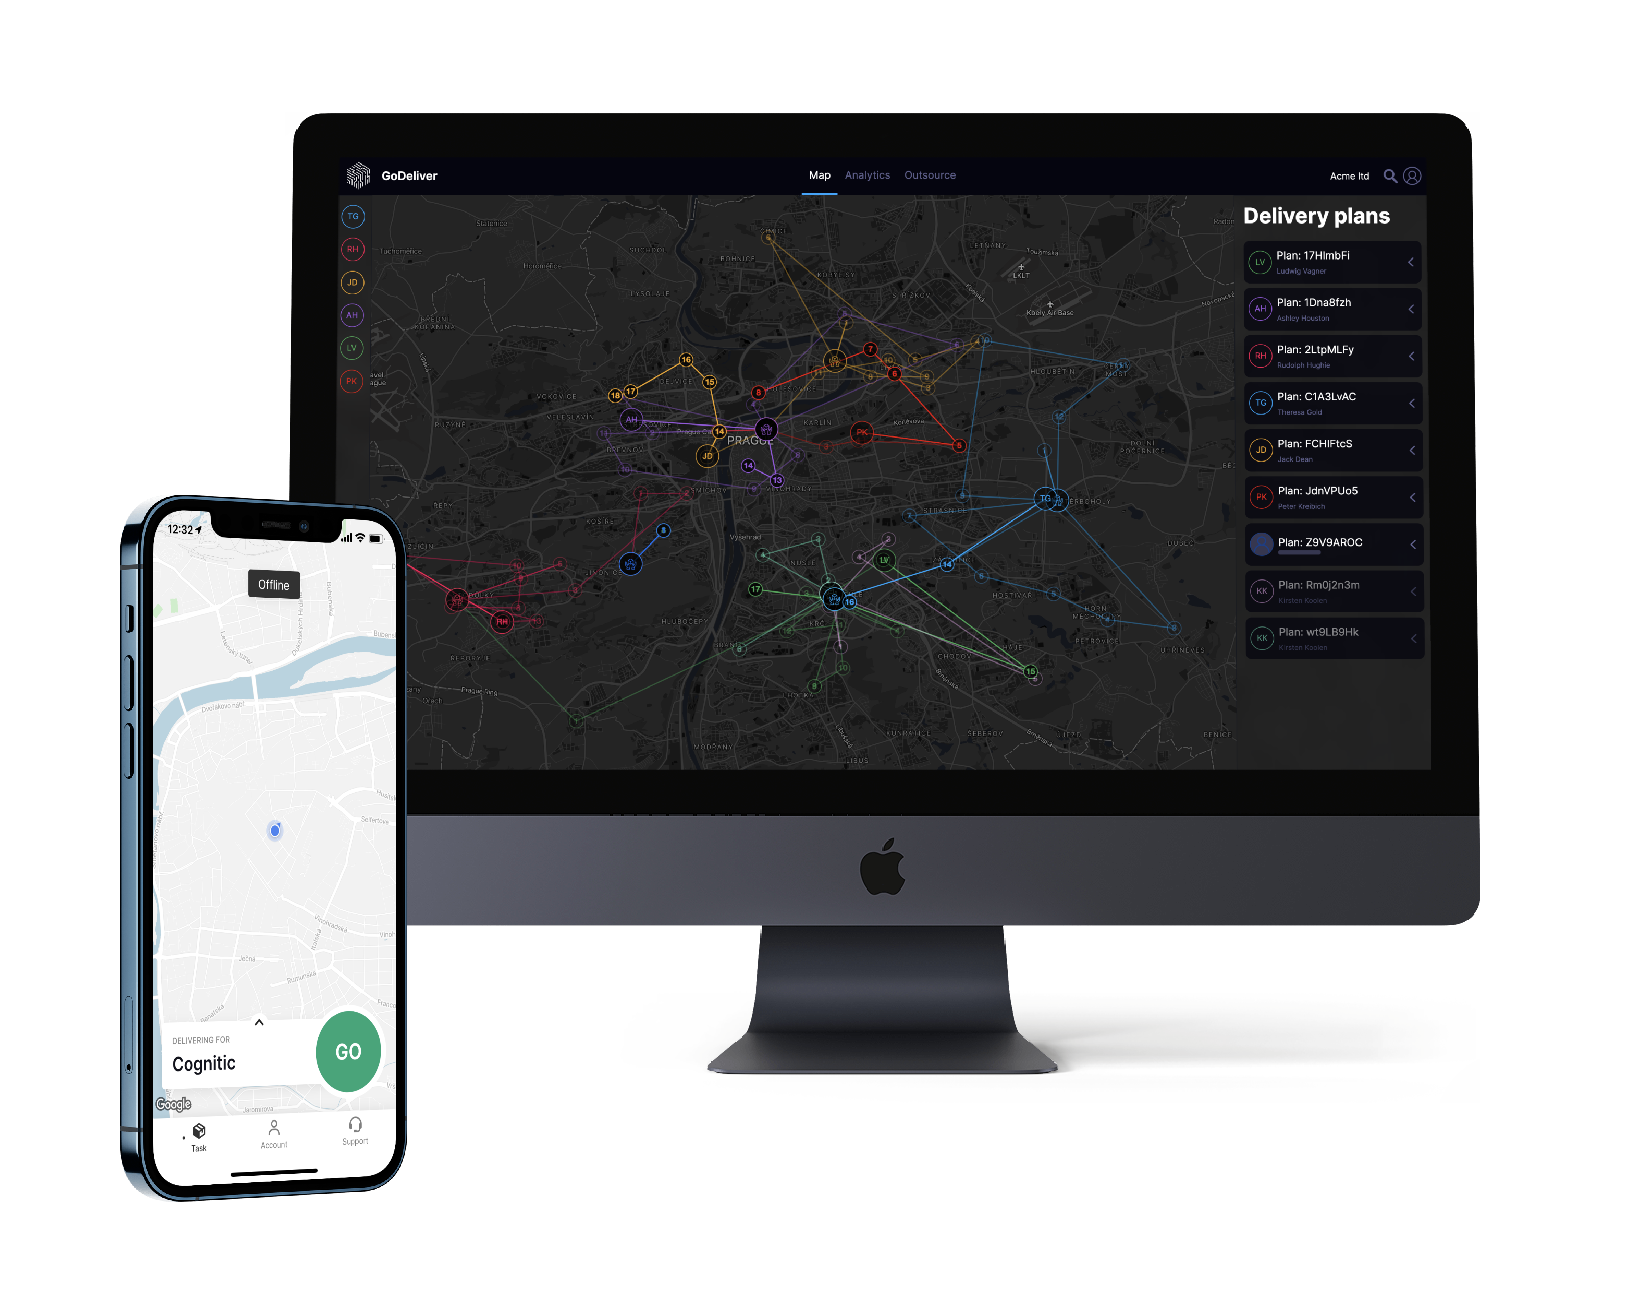
\includegraphics[width=0.8\textwidth]{figures/godeliver-system.pdf}
    	\caption[GoDeliver driver application and real-time tracking dashboard]{GoDeliver driver application and real-time tracking dashboard}
    	\label{fig:dashboard}
    \end{figure}

    \subsection{Features}

    	The most important features that GoDeliver provides are:
    	\begin{description}
    		
    		\item [Driver Management] The mobile application available for \emph{iOS} and \emph{Android} is used to provide information to drivers about their tasks. It shows the address of the next pickup or drop-off location along with the options to open the navigation and to call the customer. The application tracks the driver's location and sends information about completed tasks to the GoDeliver backend.
    		
    		\item [Real-time Visualization] The tracking dashboard for dispatchers and logistics managers allows to visualize deliveries, drivers, and routes, along with the estimated arrival times and delays.
    		
    		\item [Route Optimization] Probably the most critical feature of GoDeliver is the automated route planning. This is essentially the VRP solver which supports different VRP variants, depending on the customer's needs.
    		
    		\item [Automatic Dispatch] The aim of GoDeliver is to eliminate the need for human dispatchers assigning tasks to individual drivers. Therefore, automatic dispatch is a mechanism designed to tackle dynamic scenarios, where the system needs to react to new information, such as receiving or cancelling orders, changing the number of drivers, or route accidents and delays.
    	
    		\item [Customer Tracking] To ensure the best possible experience for the end customers, GoDeliver offers order tracking. This web app is sent to users via SMS message or email and shows the status of their order and the current location of the driver.
    		
    		\item [Data Visualisation] GoDeliver enables data-driven decisions by gathering and visualising data about the logistics fleet, such as delays, compound delivery costs, and other statistics.
    		
    		\item [External Integrations] To integrate GoDeliver within existing systems, the software provides a well-documented API and plugins to popular point-of-sale systems.
            
    	\end{description}


    \subsection{Architecture} \label{sec:godeliver-current-state}
    
    A simplified architecture of GoDeliver system is shown in figure \ref{fig:godeliver-architecture-old}. The  main logic behind GoDeliver is implemented in the \emph{Backend Service}. This service is a server application that communicates with the tracking dashboard and driver applications via a REST API. It also provides public endpoints for integrating with other systems. The data are stored in a Firestore Database\footnote{\url{https://firebase.google.com/docs/firestore}}. On certain events that should trigger the replanning a new Celery\footnote{\url{https://docs.celeryproject.org/}} job is created. The \emph{Replan Runner} consumes these jobs, calls the \emph{Logistics Planner} (highlighted in yellow color), and writes the produced solution to the database.
    
    The Logistics Planner is a stateless server that provides a single endpoint for planning. This endpoint consumes the instance of the VRP and produces a solution. In case that the solution cannot be found, an error is returned. To obtain the real distance and travel duration between each pair of nodes, the \emph{Planning Engine} is used. This server runs our own instance of Open Source Routing Machine (OSRM)\footnote{\url{http://project-osrm.org/}} which finds the shortest paths between two pairs of coordinates. This engine works over the Open Street Map\footnote{\url{https://www.openstreetmap.org/}} data that are regularly updated to include new routes and recent closures.
    
    The Logistics Planner internally uses Google ORTools for solving the VRP instance. As mentioned in section \ref{solvers}, ORTools is unable to solve larger instances and is thus insufficient for real-world use cases. Therefore, this thesis aims to upgrade the planning algorithm to comply with the real-world applications.

    \begin{figure}[ht]
        \centering
        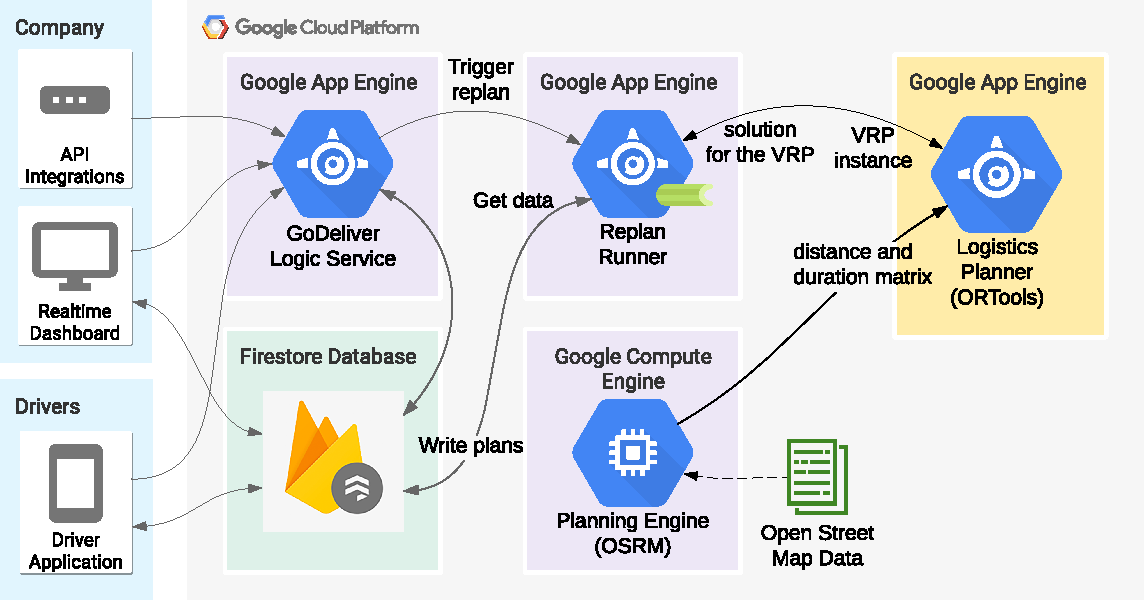
\includegraphics[width=1\textwidth]{figures/godeliver-architecture-old.pdf}
        \caption{Current state of GoDeliver architecture}
        \label{fig:godeliver-architecture-old}
    \end{figure}


\chapter{Methodology} \label{chapter:methodology}
Here, we propose a hybrid adaptive large neighborhood search algorithm for solving the problem described in the previous chapter. Next, we describe the methodology for evaluation of the proposed algorithm. Lastly, we illustrate the implementation of all mentioned parts.

\section{The Algorithm for the PDPTW} \label{sec:halns}

    The adaptive large neighborhood search (ALNS) algorithm has been successfully applied to a wide range of VRP problems, including PDPTW and DARP. In addition, the robustness of ALNS allows to efficiently solve problems with different features. However, ALNS is prone to get trapped in local optima when applied to highly constrained problems. Therefore, in this study, we combine diverse intensification strategies in the promising regions of the solution space as well as several diversification techniques to direct the search towards new and unexplored regions of the solution space. The algorithm used in this thesis is a hybrid version of ALNS, named \emph{hybrid adaptive large neighborhood search} (HALNS) and is based on the research made on DARP by primarily Masmoudi et al. (2020) \cite{Masmoudi2020}, and others, including Ropke and Pisinger (2006) \cite{Ropke2006}, Gschwind and Drexl (2016) \cite{Gschwind2016}, and Masmoudi et al. (2016) \cite{Masmoudi2016}.
    
    The majority of the ALNS algorithms in the literature uses the following approach for restarting the search: when a new solution is not better than the current solution, and is not accepted using the acceptance criterion known from the simulated annealing algorithm, the ALNS algorithm restarts the search from a solution that is generated from the same current solution by applying the removal and insertion operators. However, our algorithm does not return to the current solution. Instead, it generates a new solution using a crossover operator known from genetic algorithms. It combines the current best solution with the new solution generated by the constructive heuristics used for obtaining the initial solution. This solution is then used as the current solution. This approach gives the algorithm more diversification power as this newly generated solution is placed in a new region of the solution space, thanks to the crossover.
    
        \begin{algorithm}[!ht]
    \Input{Instance of PDPTW consisting of a set of requests and required number of drivers.}
    $ x \leftarrow InitialSolution(instance) $ \tcc*{current solution}
    $ x_{\mathrm{best}} \leftarrow x $ \tcc*{best solution}
    $ \tau \leftarrow \tau_{\mathrm{max}} $ \tcc*{temperature}
    Initialize the weights of insertion, removal, and local search operators\;
    \For{$ i \in 1,\ldots,i_{\mathrm{max}} $} {
        $x' \leftarrow$ apply removal to the current solution $ x $\;
        $x_{\mathrm{new}} \leftarrow$ apply insertion to $ x' $ \tcc*{new solution}
        
        \If{$x_{\mathrm{new}}$ is feasible} {
            \If{$cost(x_{\mathrm{new}}) < cost(x)$ or $cost(x_{\mathrm{new}})$ satisfies acceptance criterion} {
                $x \leftarrow x_{\mathrm{new}}$\;
            }
            \ElseIf{$cost(x_{\mathrm{new}}) > cost(x)$} {
                $ x_{\mathrm{init}} \leftarrow InitialSolution(instance) $\;
                $ x \leftarrow Crossover(x_{\mathrm{best}}, x_{\mathrm{init}}) $\;
            }
            \If{$cost(x_{\mathrm{new}}) < cost(x_{\mathrm{best}})$} {
                $x_{\mathrm{best}} \leftarrow x_{\mathrm{new}}$\;
                $\tau_{\mathrm{best}} \leftarrow \tau$\;
            }
            \ElseIf{$cost(x_{\mathrm{new}}) < cost(x_{\mathrm{best}})(1+\delta)$} {
                $x_{\mathrm{new}} \leftarrow LocalSearch(x_{\mathrm{new}})$\;
                \If{$cost(x_{\mathrm{new}}) < cost(x_{\mathrm{best}})$} {
                    $x_{\mathrm{best}} \leftarrow x_{\mathrm{new}}$\;
                    $\tau_{\mathrm{best}} \leftarrow \tau$\;
                }
            }
        }
        $\tau \leftarrow \alpha \tau$\;
        \If{$\tau < 0.01$} {
            $\tau_{\mathrm{best}} \leftarrow 2\tau_{\mathrm{best}}$\;
            $\tau \leftarrow min(\tau_{\mathrm{best}}, \tau_{\mathrm{max}})$\;
        }
        update the weights of insertion, removal and local search operators\;
    }
    \Return{$x_{\mathrm{best}}$}
    \caption{\label{alg:halns-loop} Hybrid Adaptive Large Neighborhood Search for PDPTW}
    \end{algorithm}
    
    
    
    Additionally, in most ALNS approaches, the best solution is updated only if the newly generated solution is better than the best solution. On the contrary, our algorithm uses an acceptance function for the new solution, which works as follows: if the newly generated solution is not worse than $\delta\,\%$ from the best solution, the new solution is not discarded. Rather, this solution is intensified using the local search procedure (see section \ref{halns:local-search}), and then compared with the best solution again. The better of the two solutions becomes the new best solution. This approach gives more chance for promising solutions to become new best solutions and thus results in more diversification power. On the other hand, using the local search procedure for promising solutions results in intensifying the search towards even better solutions.
    
    These strategies form our hybrid adaptive large neighborhood search, which combines the diversification ability of the crossover procedure and the modified acceptance function with the intensification ability of the local search procedure. Although similar approaches have been used to solve the DARP by Masmoudi et al. (2020) \cite{Masmoudi2020}, to the best of our knowledge, these novel techniques have not yet been applied to the food delivery planning problem.
    
    The main loop of our HALNS algorithm is outlined in algorithm \ref{alg:halns-loop}. Similarly to the ALNS known from Ropke and Pisinger (2006) \cite{Ropke2006}, Gschwind and Drexl (2016) \cite{Gschwind2016}, and Masmoudi et al. (2016) \cite{Masmoudi2016}, the algorithm keeps track of (1) the best solution found so far $x_{\mathrm{best}}$, (2) the current solution $x$ and (3) the newly generated solution $x_{\mathrm{new}}$. The algorithm is executed for a specified number of iterations $i_{\mathrm{max}}$ to find the best solution $x_{\mathrm{best}}$ based on its cost $cost(x_{\mathrm{best}})$ (see section \ref{halns:cost}). 
    
    In the beginning, the current solution $x$ is initialized to the new solution obtained by the construction heuristics (see section \ref{halns:init-solution}). Best solution $x_{\mathrm{best}}$ is set to the value of current solution $x$. We also initialize the temperature $\tau$ to the value $\tau_{\mathrm{max}}$ and we initialize the weights of insertion, removal, and local search operators for the adaptive weight adjustment, further described in section \ref{halns:weight}.
    
    In each iteration of the algorithm, the new solution $x_{\mathrm{new}}$ is generated from the current solution $x$ by applying the removal and insertion operators, which are described in section \ref{halns:insertion-removal}. If the best solution $x_{\mathrm{best}}$ was improved in the last iteration, one removal and one insertion operator are used to generate $x_{\mathrm{new}}$. Elseways, two removal operators and one insertion operator are used to further diversify the search. Our removal operators destroy the current solution by removing a number of requests, whereas the insertion operators repair the solution by embeding all unplanned requests back to the solution. The specific removal and insertion operators are selected based on their past performance. The selection mechanism is further described in section \ref{halns:weight}. 
    
    The new solution $x_{\mathrm{new}}$ is accepted if it is better than the current solution $x$ or if it satisfies the acceptance criterion, i.e., we accept it with probability $e^{\big(cost(x_{\mathrm{new}}) - cost(x)\big)/\tau}$. Otherwise, a new solution is obtained by utilizing a randomly selected crossover operator (see section \ref{halns:diversification}) that combines the current best solution $x_{\mathrm{best}}$ with a new solution obtained from the constructive heuristics $x_{\mathrm{init}}$ (see section \ref{halns:init-solution}). If the cost of the new solution $cost(x_{\mathrm{new}})$ is lower than the cost of the current best solution $cost(x_{\mathrm{best}})$, $x_{\mathrm{new}}$ becomes the new $x_{\mathrm{best}}$. Else, if $cost(x_{\mathrm{new}})$ is worse than $x_{\mathrm{best}}$ by a maximum of $\delta\,\%$, $x_{\mathrm{new}}$ is improved with the local search and becomes the new best solution $x_{\mathrm{best}}$ if it has lower cost compared to $x_{\mathrm{best}}$ after the intensification of the local search procedure.
    
    The temperature $\tau$, used in the acceptance criterion, is decreased in each iteration by multiplying it with the cooling rate $\alpha$. If after the cooling procedure, the temperature value becomes lower than $0.01$, $\tau_{\mathrm{best}}$, used to record the temperature when $x_{\mathrm{best}}$ is found, is multiplied by $2$ and the value of $\tau$ is set to the value of $\tau_{\mathrm{best}}$. To make sure that the search does not start from scratch from a random solution, the temperature $\tau$ is limited to $\tau_{\mathrm{max}}$.
    
    \subsection{Cost Function} \label{halns:cost}
    
    The cost function is an essential part of our HALNS algorithm as it determines the quality of the produced solution. As the costs of the intermediate solutions are measured several times in each iteration of the algorithm, especially during the application of insertion operators and our constructive heuristics, the cost function needs to be reasonably fast. Our objective is to minimize the divergence from the defined time windows and the total distance driven by the vehicles.
    
    Sometimes, it may be beneficial for the driver to arrive at the customer location before the start of the time window so that he has a lower delay for the upcoming customers. However, computing the ideal times of arrival in the plan when allowing visiting the nodes before the earliest time set by the customer would increase the complexity of the whole algorithm. To overcome this issue, we do not allow to start a service on a node before its time window starts. As a result, when the driver arrives too soon at the location, he must wait until the time window starts to begin the service\footnote{In practice, the driver may serve the customer sooner and use that extra time to compensate later delays, for example due to traffic.}.
    
    A solution $x$ consists of a set of routes $E = \{e_0,\cdots,e_k\}$, where $k$ is the number of drivers. The cost function of a single route $e \in E$ is computed as $cost(e) = \beta t^{\mathrm{delay}}_e + \gamma t^{\mathrm{distance}}_e$, where $t^{\mathrm{delay}}_e$ is the total delay of the route $e$ in seconds, $t^{\mathrm{distance}}_e$ is the total travelled distance of the route $e$ in meters, and $\beta$ and $\gamma$ are the global parameters of the algorithm (see section \ref{halns:parameters}).
    
    The total delay is computed as:
    \[ t^{\mathrm{delay}}_e = \sum_{i = 1}^{|e|-1} \max\{t^{\mathrm{eta}}_i + t^{\mathrm{service}}_i + t^{\mathrm{travel}}_{i,i+1} - w^e_{i+1}, 0\} \]
    where $t^{\mathrm{eta}}_i$ is the expected time of arrival to node $i$, $t^{\mathrm{service}}_i$ is the service time at node $i$, $t^{\mathrm{travel}}_{i,j}$ is the travel time from node $i$ to node $j$, and finally $w^e_i$ is the end of the time window of node $i$.
    
    The total distance is computed as:
    \[ t^{\mathrm{distance}}_e = \sum_{i = 1}^{|e|-1} m_{i, i+1}\]
    where $m_{i, j}$ is the travel distance between nodes $i$ and $j$.
    
    The cost of the solution $x$ is calculated as the sum of the costs of all routes, i.e., $cost(x) = \sum_{k \in K} cost(e_k)$, where $K$ is the set of drivers and $e_k$ is the route of driver $k$.

    Figure \ref{fig:plan-traversal} shows an example of traversing a single route of five nodes to compute its cost. The driver arrives at nodes 1, 3, and 5 too soon and begins the service at the start of the time window. At node 4, the driver arrives late and the difference between the end of the time window and the arrival time is the delay that is added to the total cost.
    
    \begin{figure}[ht]
        \centering
        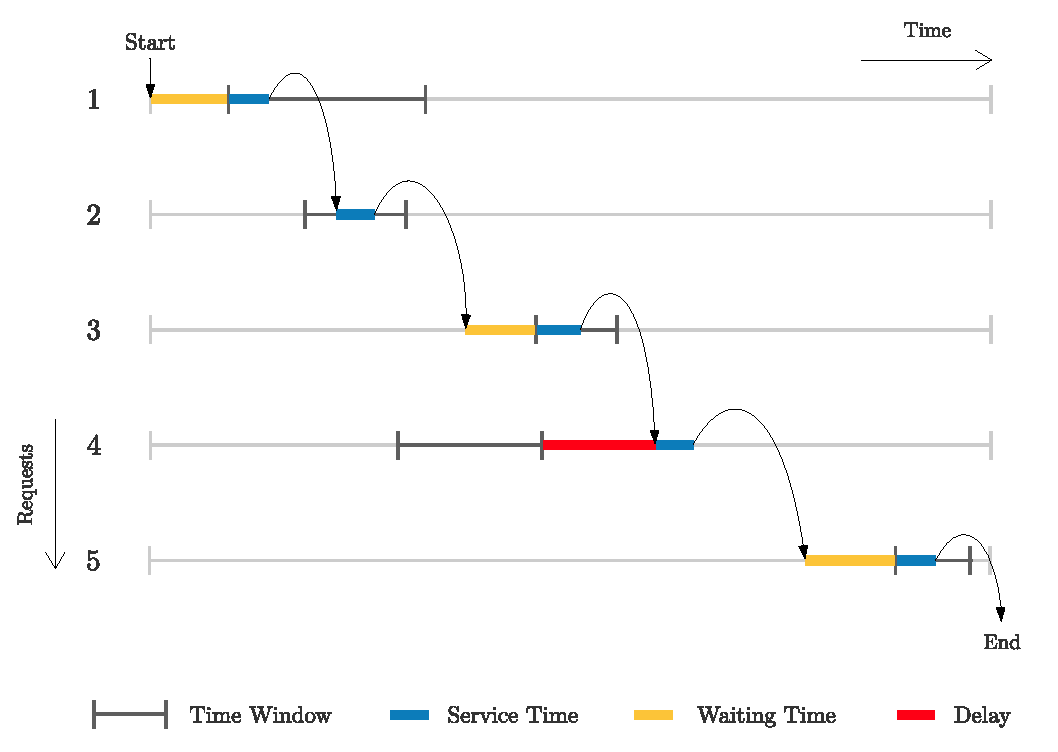
\includegraphics[width=1\textwidth]{figures/plan-traversal.pdf}
        \caption{An example of a single plan traversal for computing the cost function.}
        \label{fig:plan-traversal}
    \end{figure}
    
    
    \subsection{Removal and Insertion Operators} \label{halns:insertion-removal}
    
    The removal operators are used in each iteration to destroy the current solution by removing a number of requests from the solution and putting these requests into a set $R$. The insertion operators then repair the solution by taking the requests from the set $R$ and inserting them back into the solution, such that the solution is feasible.
    
    The removal and insertion operators were adopted from the existing literature, such as Ropke and Pisinger (2006) \cite{Ropke2006}, Pisinger and Ropke (2007) \cite{Pisinger2007}, and Demir et al. (2012) \cite{Demir2012} and adapted to our specific problem definition. The operators used in our version of HALNS are:
    
    \begin{description}
    		
    		\item [Random Request Removal (R1)] This operator randomly selects $n$ requests from the current solution $x$ and removes the corresponding pickup and drop-off nodes forming a new solution $x'$.
    		
    		\item [Path Removal (R2)] Similar to the removal operator presented by Demir et al. (2012) \cite{Demir2012}, our path removal operator randomly selects one request $r$ from the current solution $x$ and removes $n$ nodes in the plan between the pickup node $p_r$ and drop-off node $d_r$ of request $r$. We also remove all corresponding nodes such that we always remove the whole request. In other words, when only a pickup node is to be removed, we also remove the drop-off node of the same request even if it is outside of the $p_r$ and $d_r$ path.
    		
    		\item [Related Removal (R3)] This operator, based on Ropke and Pisinger (2006) \cite{Ropke2006}, randomly selects one request $r$ in the current solution and removes $n$ most related requests. The function which defines how much two requests $i$ and $j$ are related is defined as follows: $R(i,j) = m_{p_i, p_j} + m_{d_i, d_j} + \rho(|t^{\mathrm{eta}}_{p_i} - t^{\mathrm{eta}}_{p_j}| + |t^{\mathrm{eta}}_{d_i} - t^{\mathrm{eta}}_{d_j}|)$, where $p_i$ and $p_j$ (or $d_i$ and $d_j$) are the pickup nodes (or the drop-off nodes) of requests $i$ and $j$, respectively; $m_{i,j}$ is the distance between two nodes; $t^{\mathrm{eta}}_i$ is the expected time of arrival to the node $i$ in the current plan; and $\rho \in [0,1]$ is a control parameter. The operator then sorts the unplanned requests based on the function $R$ and removes $n$ requests in this order forming a new solution $x'$.
    		
    		\item [Time-oriented Removal (R4)] This operator is a special case of the related removal operator R3, where the requests that are serviced in similar times are removed. In this case, the relatedness function is defined only by the arrival times in the current solution: $R(i,j) = |t^{\mathrm{eta}}_{p_i} - t^{\mathrm{eta}}_{p_j}| + |t^{\mathrm{eta}}_{d_i} - t^{\mathrm{eta}}_{d_j}|$.
    		
    		\item [Distance-oriented Removal (R5)] This one is another special case of the related removal operator R3, where the requests in the same area as the randomly chosen request are removed. The relatedness function is defined by the distance between the pickup and drop-off nodes of the requests $i$ and $j$: $R(i,j) = m_{p_i, p_j} + m_{d_i, d_j}$.
    		
    		\item [Best Position Intra-route Insertion (I1)] This operator takes the unplanned requests from the set $R$ in a random order. For each request $r \in R$, the pickup and drop-off nodes are inserted in the first route where the insertion does not violate the feasibility. The pickup and drop-off nodes are inserted in the best possible location within the route, i.e., the cost of the insertion is the lowest possible. This is determined by checking all possible combinations of insert locations while respecting the precedence constraints. This process is repeated until $R$ is not empty.
    		
    		\item [Best Position Inter-route Insertion (I2)] This operator is similar to the intra-route operator I1, but in this case, the request $r \in R$ is inserted in the best position across all routes, rather than a single route.
    		
    		\item [Sorting Time Insertion (I3)] This operator is analogous to the intra-route operator I1, but the requests are first sorted by the start of their drop-off time window in an ascending order.
    		
    		\item [Greedy Insertion (I4)] This operator was proposed by Ropke and Pisinger (2006) \cite{Ropke2006} and is an extension of our inter-route operator (I2). Here, the requests are selected based on the insertion cost, i.e., the request that is the cheapest to insert into the solution is inserted first, and in the best possible location. This operator adds another order of time complexity, compared to the I2 operator, because to determine the insertion cost of request $r$, we need to check all possible combinations of pickup and drop-off node insertions in the solution. A known problem with this heuristic is that it postpones the insertion of expensive requests to the end, where there is not much space available.
    		
    	\end{description}
    
    In the case of removal operators, the number of requests to remove $n$ is selected from an uniform random distribution $\mathcal{U}(u_{\mathrm{min}}k, u_{\mathrm{max}}k)$, where $k$ is the number of all requests in the instance.
    
    \subsection{Local Search Procedure} \label{halns:local-search}
    
    To enhance the quality of solutions, three local search operators are used. These are inspired by the existing literature and adapted to our problem:
    
    \begin{description}
    		
    		\item [Intra-route relocate operator (L1)] This operator, adopted from Savelsbergh (1992) \cite{Savelsbergh1992}, operates on a random route in the solution. For each request $r$ in the route it removes the pickup $r_p$ and drop-off nodes $r_d$ and reinserts them back into the route in the cheapest fashion, similarly to the insertion intra-route operator I1.
    		
    		\item [Inter-route relocate operator (L2)] This operator is a special case of the previous operator L1, where the best insertion position is searched for in all plans in the solution, rather than the same route. Thus, this operator relocates requests between routes.
    		
    		\item [2-opt operator (L3)] This operator, inspired by Lin (1965) \cite{Lin1965}, takes a random route from the solution and two positions $p$ and $q$ within the plan. It then reverses the order of the nodes between the points $p$ and $q$. Because this operation might break the precedence constraints, a fixing procedure is then applied. This procedure iterates through the edited plan and swaps all pairs of pickup and drop-off nodes that are not in the correct order. All combinations of positions $p$ and $q$ are tested and the resulting solution with the lowest cost is returned.
    		
    \end{description}
    
    The local search operators can only improve the current solution and cannot generate a new solution with higher cost. During the search, these operators are selected based on the first improvement strategy, which works as follows: The current operator is applied repeatedly until no further improvements are possible, then the next operator is applied. When all local search operators were used and the solution is no longer improved, the procedure ends and the current solution is returned.
    
    In addition, the specific local search operators are selected based on their past performance using a roulette wheel mechanism, which is further described in section \ref{halns:weight}.
    
    \subsection{Adaptive Weight Adjustment} \label{halns:weight}
    
    In section \ref{halns:insertion-removal} we defined five removal operators and four insertion operators. Additionally, section \ref{halns:local-search} defined three local search operators. Similarly to other ALNS algorithms from the literature, we propose to use all these operators during the search. The reason behind this is that while one specific operator might be well suited to one type of instance, others might perform better on different types of instances. As a consequence, alternating between these operators results in a more robust algorithm. The adaptive weight adjustment procedure defined in this section is inspired by Ropke and Pisinger (2006) \cite{Ropke2006}.
    
    The operators are selected according to their past performance during the search. Each operator in its respective category is assigned a weight and the specific operator is selected in each iteration using a roulette wheel mechanism. The whole search is divided into \emph{segments}, which is the number of iterations of the algorithm; here we define the segment as 100 iterations ($n_{seq} = 100$).
    
    The probability of choosing an operator $d$ in iteration $t$ is given by: $P^t_d = P^{t-1}_d (1-r_p) + r_p \pi_d / \omega_d$, where $r_p$ is the roulette wheel parameter, $\pi_d$ is the score of the operator $d$ in the last segment, and $\omega_d$ is the counter of how many times the operator $d$ was used in the last segment. The initial probabilities $P^0_d$ are constants defined in section \ref{halns:parameters}.
    
    The scores of the operators are set to $0$ at the beginning of each segment. They are increased in each iteration depending on their performance: we increase the score by $\pi_1$ if the operator finds a new best solution $x_{\mathrm{best}}$, by $\pi_2$ if the operator improves the current solution $x$, and finally by $\pi_3$ if the operator finds a feasible solution that is worse than the current solution $x$ but is accepted via the acceptance criterion. At the end of the segment, the weights are adjusted based on the values defined above and the counts $\omega$ are set to $0$;
    
    The reasoning behind $\pi_1$ is clear: when an operator finds a new best solution $x_{\mathrm{best}}$, it has done well. Similarly, if the operator finds a solution that is accepted by the acceptance criterion, it is also successful as it advances the search. We distinguish between the situations which correspond to the parameters $\pi_2$ and $\pi_3$ as we prefer the operators that improve the solution, however, we are also interested in diversifying the search.
    
    \subsection{Initial Solution} \label{halns:init-solution}
    
    The constructive heuristic that provides the initial solution at the beginning of the algorithm, and later for the crossover operation is an \emph{insertion heuristic} adopted from Lu and Dessouky (2006) \cite{insertionHeuristics}. The algorithm \ref{alg:insertion-heuristic} shows how the insertion heuristic works in our context. The functionality of this algorithm is analogous to the inter-route insertion operator I2, defined in section \ref{halns:insertion-removal}, but in this case, all requests are to be inserted into an initially empty solution.
    
    
    \begin{algorithm}[!ht]
    \Input{The set of unplanned requests $R$ and the list of drivers $K$}
    shuffle the requests in $R$\;
    \For{request $r \in R$}{
        \For{driver $k \in K$}{
            let $e_k$ be a current route of driver $k$\;
            let $l$ be the length of route $e_k$
            \For{$i \in 1,\ldots,l+1$}{
                \For{$j \in i+1,\ldots,l+2$}{
                    $e_k' \leftarrow$ insert \texttt{pick-up(r)} before position $i$ in plan $e_k$\;
                    $e_k^{i,j} \leftarrow$ insert \texttt{drop-off(r)} before position $j$ in plan $e_k'$\;
                }
            }
        }
        $k^*, i^*, j^* \leftarrow \underset{k, i, j}{arg\,min}\; cost(e_k^{i,j}) - cost(e_k)$ subj. to $e_k^{i,j}$ is feasible\;
        request $r$ is inserted into the route of driver $k^*$, pickup node before position $i^*$ and drop-off node before position $j^*$.\;
    }
    \caption{Insertion heuristics for creating an initial solution for our HALNS algorithm}
    \label{alg:insertion-heuristic}
    \end{algorithm}
    
    
    \subsection{Diversification Mechanism} \label{halns:diversification}
    
    To explore the unknown regions of the solution space and thus provide the algorithm with more diversification capability, the crossover mechanism described above is applied during the search. The operation combines the current best solution $x_{\mathrm{best}}$ with an initial solution $x_{\mathrm{init}}$ constructed by the constructive heuristic (see section \ref{halns:init-solution}). The intention of this operation is to find approximately the same quality solution that is placed in a different region of the solution space. Three different crossover operators that are well-known from the literature on genetic algorithms are used. The visualisation of the usage of these operators on an example route is shown in figure \ref{fig:crossover}.
    
    \begin{figure}[!hb]
        \centering
        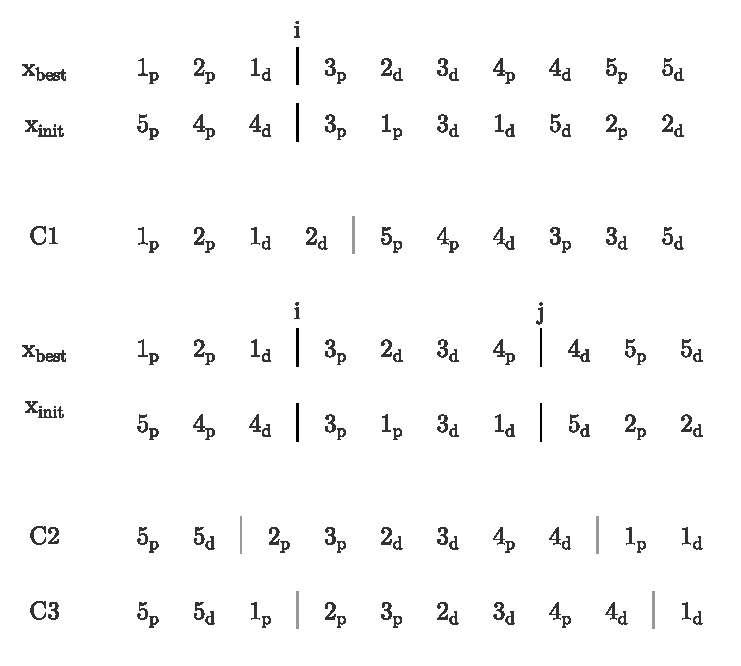
\includegraphics[width=0.9\textwidth]{figures/crossover.pdf}
        \caption{A visualisation of the three crossover operators.}
        \label{fig:crossover}
    \end{figure}
    
    \begin{description}
    		
    		\item [One-point Crossover (C1)] This operator is inspired by Prins (2004) \cite{Prins2004}, who applied this operator to instances of classical VRP. In our usecase of PDP, the operator works as follows: first, a random position $i$ is selected, such that $0 < i < \max_{k \in K}{|e_k|}$, where $K$ is the set of drivers, $e_k$ is the route of driver $k$, and $|e_k|$ is its length. Second, all requests whose node appears before position $i$ in each route of $x_{\mathrm{best}}$ are copied to the new solution in their respective order. Finally, the rest of the requests are copied from $x_{\mathrm{init}}$ in the respective order, skipping the requests that are already in the new solution.
    		
    		\item [Two-point Crossover (C2)] A similar operator was proposed by Goldberg and Holland (1988) \cite{Goldberg1988}. In our case, two positions $i$ and $j$ are selected, such that $0 < i < j < \max_{k \in K}{|e_k|}$. The operator copies all requests, whose nodes appear between positions $i$ and $j$ in routes from $x_{\mathrm{best}}$ to the new solution while maintaining their order. Finally, the same operation is performed on nodes that appear before position $i$ and after position $j$ in routes from $x_{\mathrm{init}}$, but in reverse order.
    		
    		\item [Linear Two-point Crossover (C3)] This operator, proposed by Sevaux and Dauzère-Pérès (2003) \cite{Sevaux2003} is similar to the two-point crossover operator C2. The only difference is that after copying the nodes from $x_{\mathrm{best}}$, the rest of the nodes are copied from $x_{\mathrm{init}}$ in their respective order. After that, to ensure the precedence constraints are satisfied, a repair procedure which adds the nodes of the incomplete requests is performed.
    		
    \end{description}
    

    
    \subsection{Parameter Selection}\label{halns:parameters}
    
    The parameters mentioned throughout the algorithm description are summarized and explained in this section. Generally, the parameters are selected based on the proposals and experimental results from the literature, such as  Ropke and Pisinger (2006) \cite{Ropke2006}, Demir et al. (2012) \cite{Demir2012}, Leung et al. (2013) \cite{Leung2013}, and Masmoudi et al. (2016, 2020) \cite{Masmoudi2016, Masmoudi2020}. Three parameters were not adopted from the literature and are based on our experiments. These are the maximum number of iterations $i_{\mathrm{max}} = 100\,000$, in which we observed that the solution is no longer improving on our evaluation dataset; and the coefficients of total delay $\beta = 1$ and total distance $\gamma = 0.5$ in the cost function, which seem to be a good balance between prioritizing the user satisfaction and minimizing the operational cost. Table \ref{tab:parameters} summarizes the parameters used in our algorithm.
    
    \begin{table}[!ht]
    \centering
    {\renewcommand{\arraystretch}{1.5}
    \begin{tabular}{llll}
    \hline
    \textbf{Not.}          & \textbf{Description}                            & \textbf{Value} & \textbf{Source}             \\ \hline
    $i_{\mathrm{max}}$     & Maximum number of iterations                    & $100\,000$       &                             \\
    $\beta$                & Coefficient of delay in cost calculation        & $1$            &                             \\
    $\gamma$               & Coefficient of distance in cost calculation     & $0.5$          &                             \\
    $n_{seq}$              & Num. of iterations to update the weights        & $100$          & \cite{Masmoudi2016}         \\
    $u_{min}$              & Min. \% of requests removed at each iteration   & $0.175$        & \cite{Pisinger2007}         \\
    $u_{\mathrm{max}}$     & Max. \% of requests removed at each iteration   & $0.35$         & \cite{Pisinger2007}         \\
    $r_p$                  & Roulette wheel parameter                        & $0.7$          & \cite{Masmoudi2016}         \\
    $P^0_{r}$              & Initial probability of removal operators        & $0.1$          & \cite{Masmoudi2016}         \\
    $P^0_{i}$              & Initial probability of insertion operators      & $0.125$        & \cite{Masmoudi2016}         \\
    $P^0_{ls}$             & Initial probability of local search operators   & $0.125$        & \cite{Masmoudi2016}         \\
    $\pi_{1}$              & Score of a new best solution                    & $15$           & \cite{Masmoudi2020}         \\
    $\pi_{2}$              & Score of a new current solution                 & $10$           & \cite{Masmoudi2020}         \\
    $\pi_{3}$              & Score of a feasible non-improving solution      & $5$            & \cite{Masmoudi2020}         \\
    $\tau_{\mathrm{max}}$  & Initial temperature                             & $25$           & \cite{Leung2013}            \\
    $\alpha$               & Cooling rate                                    & $0.99975$      & \cite{Ropke2006, Demir2012}

    \end{tabular}
    }
    \caption{The parameters used in our HALNS algorithm}
    \label{tab:parameters}
    \end{table}
    
\section{Methods for Evaluation}
    
    To evaluate the performance of the HALNS algorithm described in the previous section, three important components were needed. Firstly, we created datasets with different instances of the problem, i.e., with different number of requests and drivers. Secondly, we constructed a baseline algorithm for comparison with the newly developed HALNS algorithm. Lastly, we defined the metrics to be used for evaluating both the baseline and the HALNS algorithms.

    \subsection{Evaluation Datasets} \label{sec:dataset}
    
    Evaluation datasets contain different sizes of the problem instances. To create these datasets, we used real data from a selected company, which delivers food from seven restaurants in Prague. The data that could match the order details to specific customers were removed to keep anonymity.
    
    For each request, the collected data relevant to our purposes are the following:
    
    \begin{enumerate}
        \item Pickup Location
        \item Drop-off Location
        \item Pickup Time Window
        \item Drop-off Time Window
        \item Order Creation Time
        \item Number of Packages
    \end{enumerate}

     To create the different instances, we took all requests from this company since the 1\textsuperscript{st} of January 2020 until the 5\textsuperscript{th} of May 2020, totalling 7\,100 requests. Next, all time windows of these requests were shifted to a single day. Figure \ref{fig:dataset-map} shows a distribution of the coordinates on the map of Prague. The distribution of the starts of the time windows at drop-off locations of these requests is shown in figure \ref{fig:dataset-distribution}. It is clear that the vast majority of all deliveries should be delivered between 11 AM and 1 PM.
    
    \begin{figure}[!ht]
        \centering
        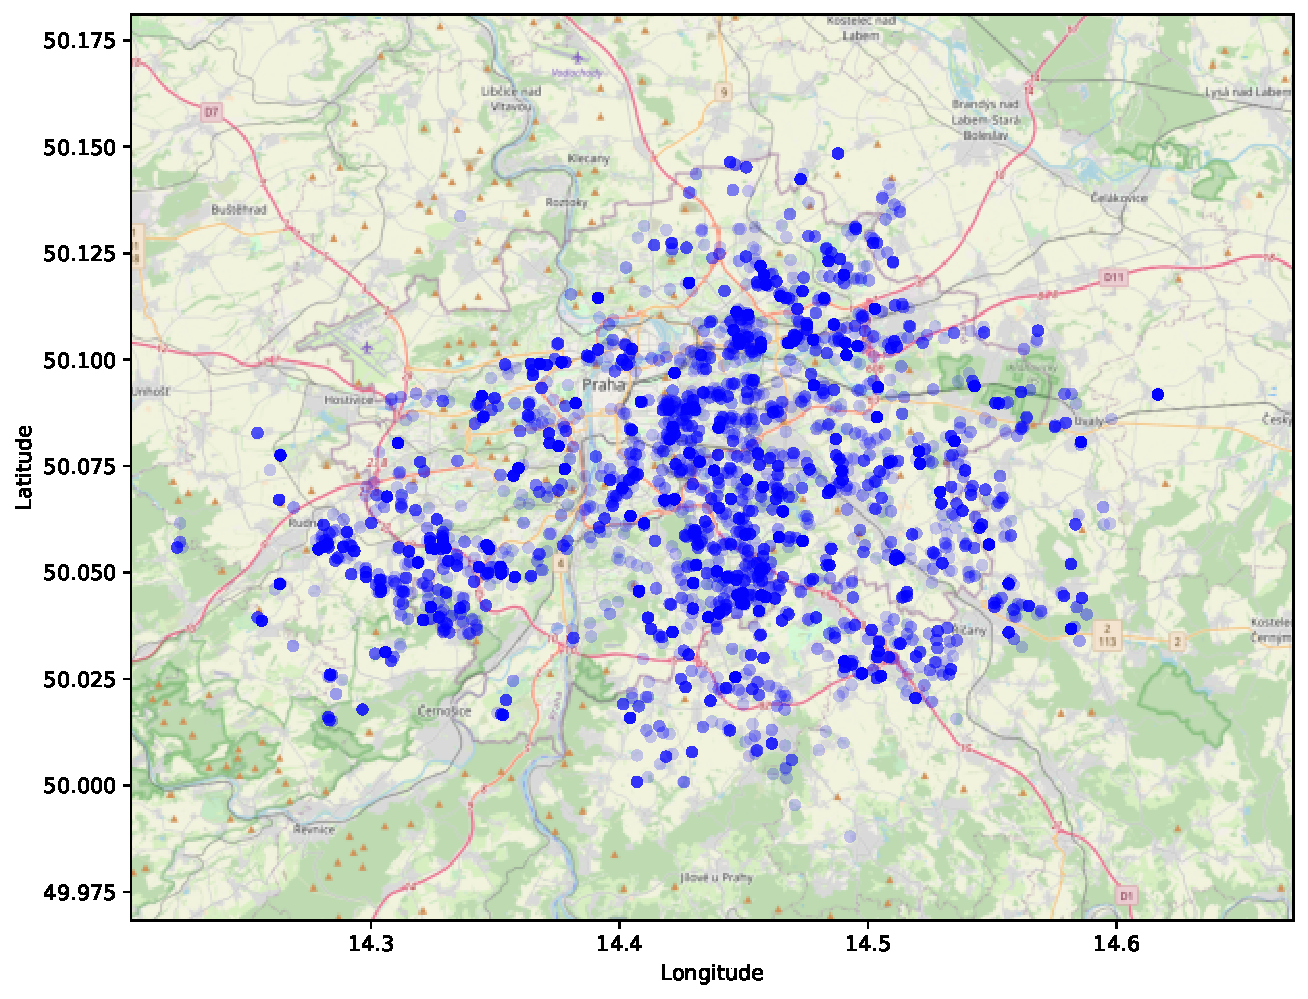
\includegraphics[width=\textwidth]{figures/dataset-map.pdf}
        \caption{A distribution of drop-off locations in the full request dataset of 7\,100 requests.}
        \label{fig:dataset-map}
    \end{figure}
    
    \begin{figure}[!ht]
        \centering
        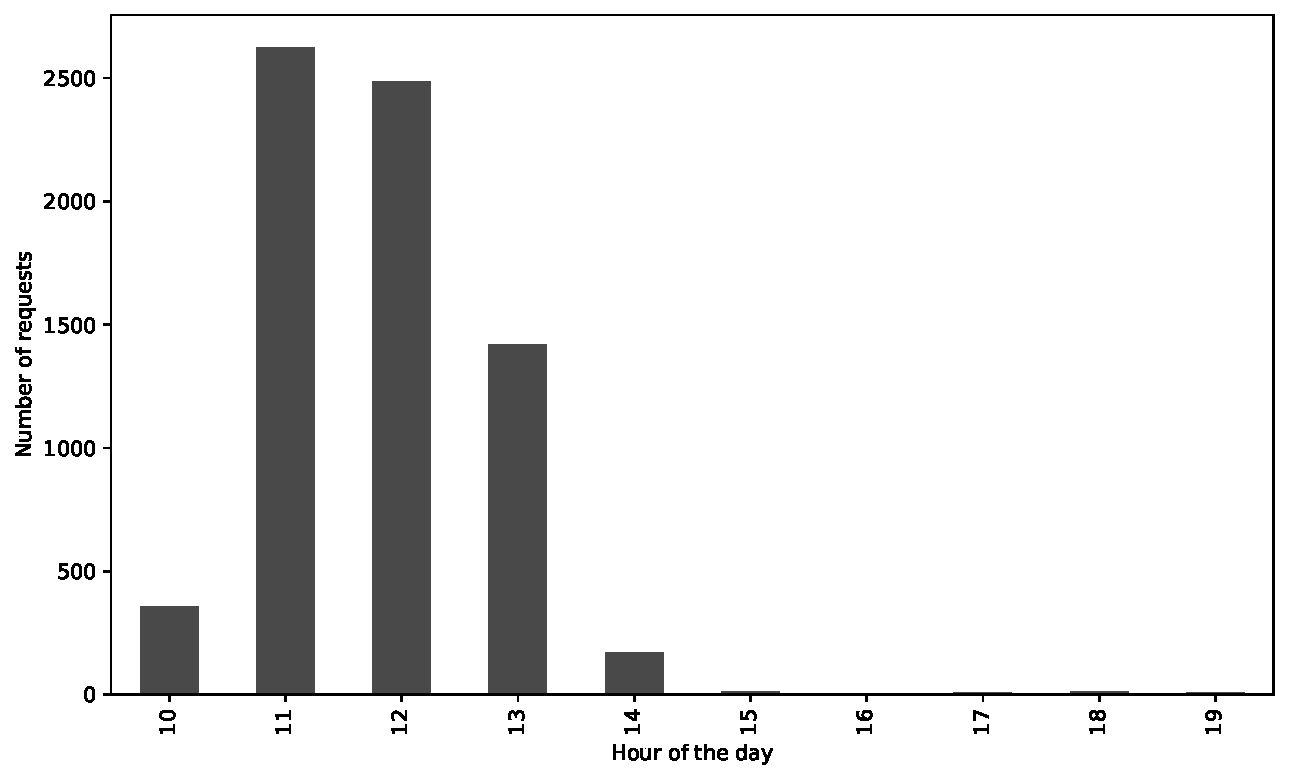
\includegraphics[width=\textwidth]{figures/dataset-distribution.pdf}
        \caption{A distribution of the earliest times of drop-off set by the customers throughout the day in the full request dataset of 7\,100 requests.}
        \label{fig:dataset-distribution}
    \end{figure}

    The individual instances were created by selecting random subsets of different sizes from this set. We used five different instance sizes and prepared 10 instances of each size. For each of these instance sizes, the number of drivers was determined. Based on the distribution of time windows in figure \ref{fig:dataset-distribution}, most requests arrive in a period of 2.5 hours. Additionally, based on our experiments with our current ORTools planner, a single driver is able to finish 3.5 requests per hour. Thus, the number of drivers is computed as $\mathrm{round}(\frac{|r|}{2.5\,3.5})$, where $|r|$ is the number of requests in the instance.
    
    To sum up, 10 different random instances of each of the following sets were prepared. They are shown in table \ref{tab:datasets}.
    
    \begin{table}[!ht]
    \centering
    {\renewcommand{\arraystretch}{1.5}
    \begin{tabular}{lll}
    \hline
               & \textbf{Requests} & \textbf{Drivers} \\ \hline
    \textbf{1} & 20                & 2                \\
    \textbf{2} & 50                & 6                \\
    \textbf{3} & 100               & 11               \\
    \textbf{4} & 200               & 22               \\
    \textbf{5} & 500               & 56              
    \end{tabular}}
    \caption{5 evaluation datasets, each containing 10 different instances}
    \label{tab:datasets}
    \end{table}

    
    \subsection{Baseline Algorithms} \label{sec:baseline}
    
    As a baseline, three methods were used. The first is a simple insertion heuristic, as was used for constructing an initial solution for the HALNS algorithm and is described in section \ref{halns:init-solution}. The second is the ORTools planner that is already part of the GoDeliver system and is described in section \ref{sec:godeliver-current-state}. The last one combines the insertion heuristic with the ORTools planner, first creating the solution using the insertion heuristic, and using that solution as an initial solution for the ORTools planner for improvement. This approach overcomes the problem that ORTools is unable to find an acceptable solution on larger instances. These three methods are visualised in figure \ref{fig:baseline-algorithms}.
    
    \begin{figure}[!ht]
        \centering
        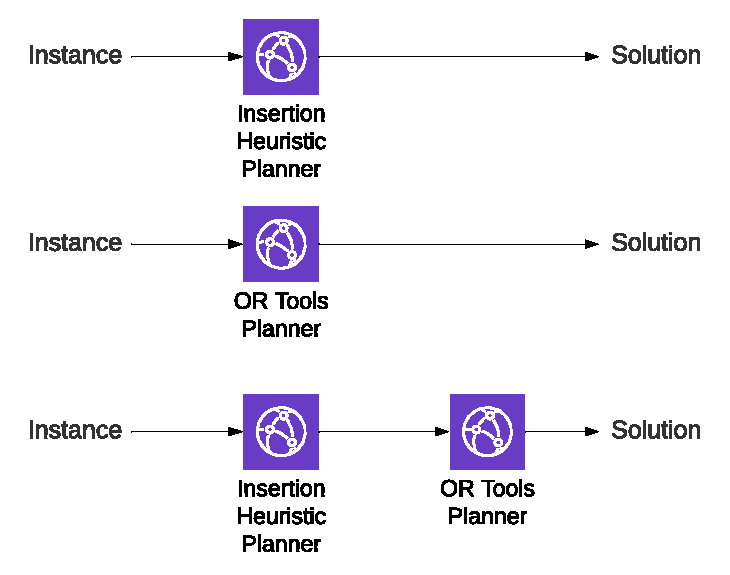
\includegraphics[width=0.8\textwidth]{figures/baseline-algorithms.pdf}
        \caption{Three baseline algorithms for evaluating the performance of our HALNS algorithm.}
        \label{fig:baseline-algorithms}
    \end{figure}
    
    \subsection{Metrics} \label{sec:metrics}
    
    For problem instances of more than a few tens of requests, it is nearly impossible to find the optimal solution. In addition, the cost of the solution alone does not reveal the full information about the solution quality. For these reasons, we defined the metrics that help us evaluate the solutions produced by different algorithms. These metrics indicate how good the produced solutions are with respect to our objectives.

    These metrics include:
    \begin{description}
        \item[Delay of Drop-off (M1)] This is probably the most important metric that best describes the customer satisfaction constraint. It indicates the time difference between the drop-off time window and the estimated time of arrival of the drivers. We measure the average and the maximum delay per request. 
        
        \item[Total Distance Travelled (M2)] This is the second most important metric which shows the optimality of the routes with respect to the cost of delivery. It is defined as the sum of the total distance travelled by all drivers.
        
        \item[Total Time Spent (M3)] This metric is an addition to the previous metric M2. It indicates the total time spent on the route across all couriers. We assume a high correlation between this metric and the M2 metric, since the distance is directly proportional to the driving time. However, this metric also includes the waiting times at the nodes and thus might produce different results.
                
        % \item[Delay of Pickup (M4)] Similarly to the M1 metric, we measure the time difference between the pickup time window and the estimated time of arrival of the drivers. This metric does not relate too much to customer satisfaction, but contributes to the wuality of the service.

        % \item[Number of Deliveries per Driver (M4)] This metric indicates how many requests were handled by a single driver. While the average will always be the same, i.e., $|r|/|K|$, where $|r|$ is the number of requests and $|K|$ is the number of drivers, the maximum and minimum numbers can reveal either insufficient or excessive number of drivers.
        
        \item[Delivery En Route Time (M4)] This metric shows the duration of a single delivery between its pickup and drop-off estimated times. In other words, it shows how long is the delivery (in our case the food) in the vehicle before it is delivered. This is especially important for perishables, such as ready-to-eat meals.
        
        \item[Delivery Load (M5)] This metric indicates how well the algorithm is able to stack the requests within the route, i.e., it is the average number of orders picked up by the driver at one location.
        
    \end{description}

\section{Implementation}
    
    This section describes the implementation details of the planning algorithm and its integration into GoDeliver pipeline. It also briefly illustrates the developed evaluation environment that is also part of this thesis.
    
    \subsection{Planning Algorithm}
    
    The main HALNS algorithm described in section \ref{sec:halns} as well as the insertion heuristics baseline mentioned in section \ref{sec:baseline} were implemented in \emph{Go} language\footnote{\url{https://golang.org/}} version \emph{1.15.8}. We opted for Go primarily for these reasons: it is a statically typed, compiled language and thus much more performant compared to, for example, Python; it has great support for concurrency which allows to speed up the algorithm even more; it is easy to create compiled binaries for all operating systems which makes the continuous integration pipeline easy; and finally there is a large community around Go which contributes to our confidence in its further development and support.
    
    The most critical entity in the whole algorithm is the \texttt{solution} structure that is constantly being destroyed by removal operators, repaired by insertion operators, improved by the local search procedure, and combined with a new solution by applying the crossover mechanism. The solution instance keeps the list of $n$ \texttt{plans}, where $n$ is always the required number of drivers, and a set of unplanned \texttt{requests}, i.e., the requests that are not part of the solution, for example, after the removal operator is applied. Each plan contains a list of \texttt{actions}. Actions represent the graph nodes of a specific type. An action can be of three types: start, pickup, and drop-off. Each request contains one or two actions, depending on whether the request is already picked up before the planning procedure starts (see section \ref{sec:dynamicity}). In the static variant, a single request contains exactly two actions: pickup and drop-off. For better understanding, figure \ref{fig:entity-diagram} reveals the relationships between these entities.
    
    \begin{figure}[!ht]
        \centering
        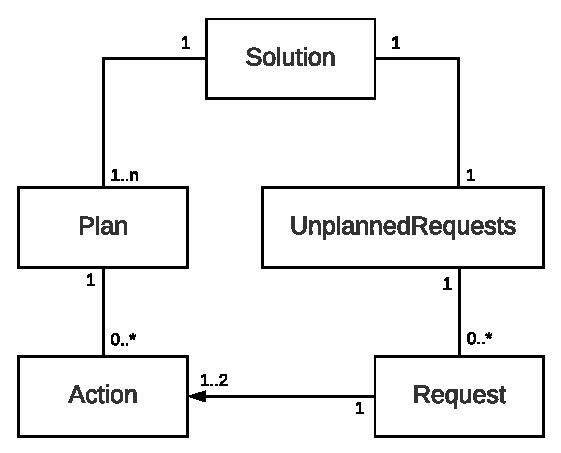
\includegraphics[width=0.6\textwidth]{figures/entity-diagram.pdf}
        \caption{A simplified entity relationship diagram of the data model used in Go implementation.}
        \label{fig:entity-diagram}
    \end{figure}
    
    
    Because Go works with the concept of interfaces rather than inheritance, so typical for other languages, the architecture of the algorithm is notably shaped by this concept. We define four interfaces for the operators used: removal, insertion, local search, and crossover. Each of these interfaces defines a different signature for the \texttt{Apply} method, that applies the operator and produces a new solution. For example, the removal operators accept two parameters: the current solution and the number of requests to remove, whereas the crossover operators need to be provided with two solutions as parameters. These interfaces are shown in figure \ref{fig:operators-diagram}.

    
    \begin{figure}[!ht]
        \centering
        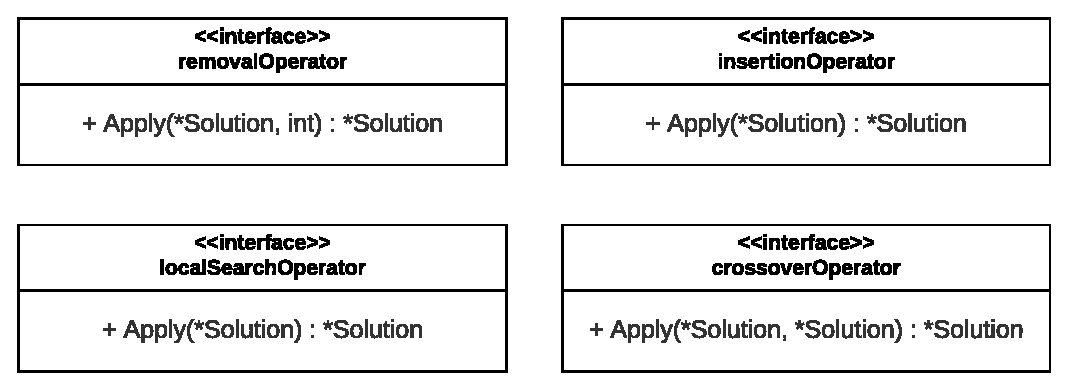
\includegraphics[width=0.8\textwidth]{figures/operators-diagram.pdf}
        \caption{Four operator interfaces used in the Go implementation of the HALNS algorithm.}
        \label{fig:operators-diagram}
    \end{figure}  
    
    \subsection{Integration into GoDeliver Pipeline}
    
    Extensive work was done on the integration part. The previous state of the GoDeliver Planner Service is described in section \ref{sec:godeliver-current-state}. The service was tightly coupled with the ORTools solver and was not extendable nor easily testable. Therefore, we abstracted the individual planning algorithms (baseline and HALNS) into their respective classes, which extend the \texttt{AbstractPlanner} class. This class is now responsible for serializing the instance, calling the respective planner, and deserializing the solution. Since the HALNS and insertion heuristics planners are implemented in Go, the GoDeliver Planner Service loads an already compiled binary as a C library, which can be called from Python. The class diagram of \texttt{AbstractPlanner} class and its subclasses is shown in figure \ref{fig:abstract-planner-diagram}.
    
    \begin{figure}[!ht]
        \centering
        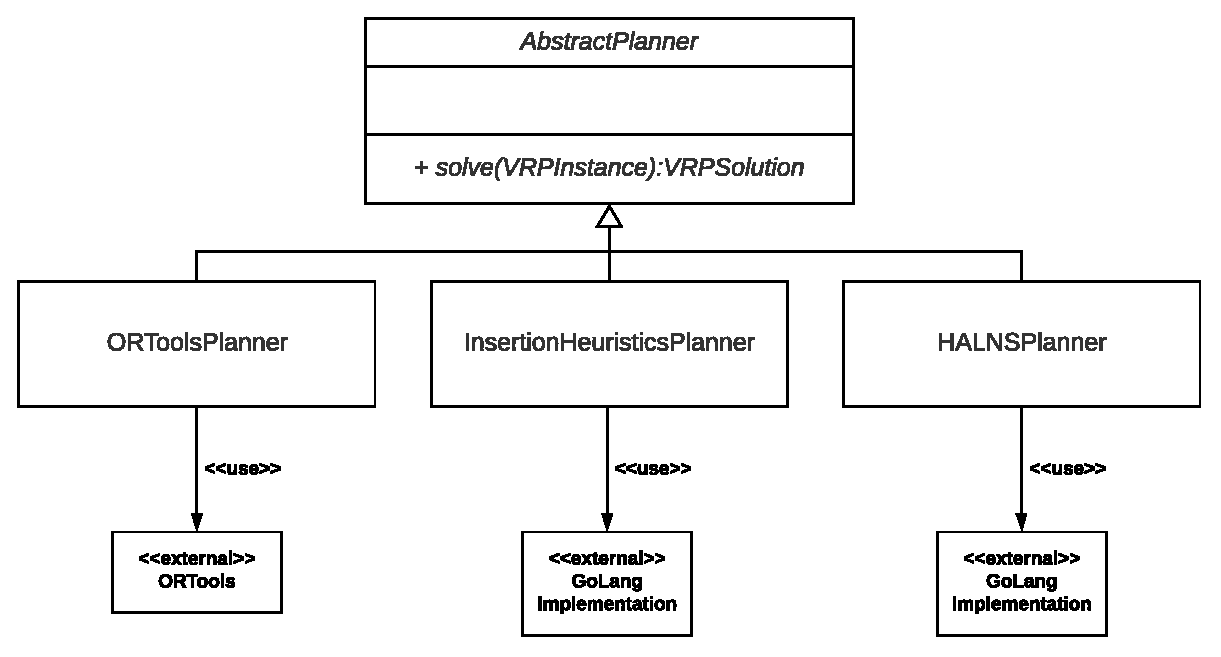
\includegraphics[width=0.8\textwidth]{figures/abstract-planner-diagram.pdf}
        \caption{The Abstract Planner class, and three specific planner implementations in GoDeliver Planner.}
        \label{fig:abstract-planner-diagram}
    \end{figure}  
    
    In addition to this abstraction, we introduced a way to easily benchmark these planning algorithms and visualize the produced solutions and metrics. For that, we use \emph{plotly}\footnote{\url{https://plotly.com/}} framework for visualizing the plans and \emph{streamlit}\footnote{\url{https://streamlit.io/}} framework that displays the metrics of all methods in a simple and understandable way. Figure \ref{fig:godeliver-architecture-new} displays the improved and extensible architecture of GoDeliver Planner Service.
    
    \begin{figure}[!ht]
        \centering
        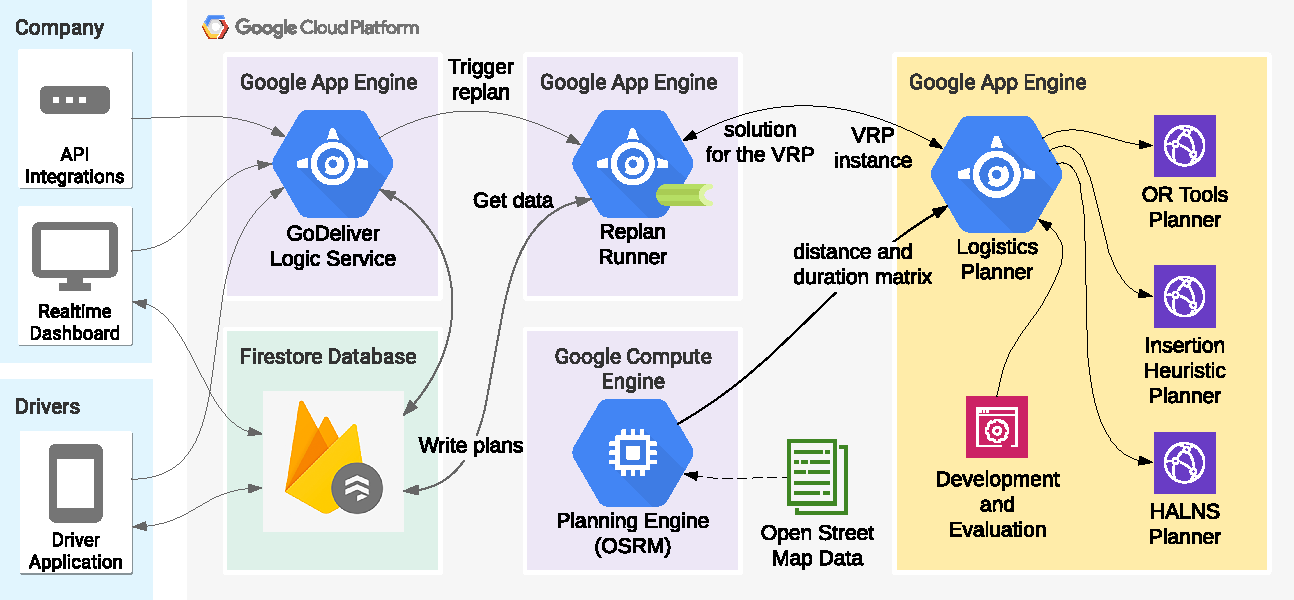
\includegraphics[width=1\textwidth]{figures/godeliver-architecture-new.pdf}
        \caption[The new architecture of GoDeliver Planner.]{The new architecture of GoDeliver Planner (highlighted by the yellow rectange).}
        \label{fig:godeliver-architecture-new}
    \end{figure}
    

\chapter{Results} \label{chapter:results}
This chapter shows the experimental results of our proposed HALNS algorithm in comparison with the defined baseline methods. It also analyzes the adaptive weight adjustment and details the parameter selection process.

\section{Experimental results}

    Here, we compare our proposed HALNS algorithm described in section \ref{sec:halns} with the three baseline methods detailed in section \ref{sec:baseline}. The experiments were conducted on the benchmark datasets, which are illustrated in section \ref{sec:dataset}. Each dataset consists of 10 instances with the same number of requests and drivers. Each experiment on each instance was executed 10 times and the results were averaged. All experiments were conducted on a machine with a 2,6 GHz 6-Core Intel Core i7 processor and 16 GB of RAM, and the maximum running time was restricted to 10 minutes. The ORTools baseline method is unable to reasonably solve instances containing more than 20 requests. Therefore, the ORTools method was evaluated only on the smallest instance containing 20 requests.
    
    For comparison of the algorithms, we use the metrics M1 to M5 introduced in section \ref{sec:metrics} rather than the objective value. The reason is that these metrics provide much deeper insight into the quality of the produced solutions. Table \ref{tab:delay} contains the experimental results in the context of the M1 metric, which indicates the average (and maximum) delay per single request at its drop-off location. Similarly, Table \ref{tab:distance} highlights the M2 metric results, which indicates the average (and maximum) distance driven by each driver. In both tables, the minimum values are in bold to feature the best algorithm per each dataset. All five metrics M1 to M5 are then visualized in figure \ref{fig:metrics-graphs}. For each metric, we show the average value per each dataset and method along with the standard deviation. In the mentioned tables and figures, \emph{IH} stands for insertion heuristics baseline method, and \emph{IH \& ORTools} refers to the combination of insertion heuristics and ORTools, which is one of the baseline methods described in section \ref{sec:baseline}.

    The results in tables \ref{tab:delay} and \ref{tab:distance} show that the HALNS algorithm is significantly better regarding the delay and distance compared to the baseline methods on bigger instances. In contrast, on the smallest instance of 20 requests, the HALNS algorithm produces slightly worse results than insertion heuristics in combination with ORTools in terms of both metrics, however, it has slightly lower standard deviation.
    
    From the table \ref{tab:delay} we may observe much worse delays in the smallest instances, especially the maximum values. The reason behind it is the small number of drivers (two drivers used in each instance), which results in much more travelling as each driver needs to service larger areas. As a consequence, larger travel times produce larger delays.
    
    The ORTools planner alone produces the worst solution in terms of delays on the 20 request dataset and has the largest deviation. In terms of total distance, ORTools outperforms HALNS and insertion heuristics.
    
    The maximum values of the delay and distance shown in tables \ref{tab:delay} and \ref{tab:distance} suggest that HALNS is able to equally distribute the delays and distance between the requests and drivers, respectively.
    
    There is a strong correlation between the results of metrics M2 and M3 - the distance driven and the time spent by the drivers. In terms of the M3 metric, HALNS is comparable to the IH \& ORTools method. The metric M4, which denotes the average duration of travel per each request, is comparable for all methods.
    
    The results of the metric M5, which denotes the delivery load per each pickup, show a higher ability of the HALNS algorithm to stack the orders to increase the efficiency compared to the baseline methods on all datasets.
    
    \begin{table}[!ht]
    \centering
    {\renewcommand{\arraystretch}{1.5}
    \begin{tabular}{lllll}
    \hline
                    & \textbf{HALNS}    & \textbf{ORTools}  & \textbf{IH}         & \textbf{IH \& ORTools} \\ \hline
    \textbf{20 r.}  & 12.82 (\textbf{63.48})     & 23.49 (98.60)     & 22.89 (103.31)      & \textbf{9.32} (66.82)           \\
    \textbf{50 r.}  & \textbf{0.10} (\textbf{3.49})       &                   & 1.84 (23.10)        & 0.67 (5.98)            \\
    \textbf{100 r.} & \textbf{0.04} (\textbf{1.68})       &                   & 1.18 (22.98)        & 0.17 (8.23)            \\
    \textbf{200 r.} & \textbf{0.02} (\textbf{1.62})       &                   & 0.16 (7.50)         & 0.09 (7.08)            \\
    \textbf{500 r.} & \textbf{0.07} (\textbf{6.62})       &                   & 0.14 (11.03)        & 0.14 (9.76)
    \end{tabular}}
    \caption{Results of metric M1 - Average (and maximum) delay in minutes at drop-off locations, evaluated on our 5 datasets, averaged from 10 runs on each instance.}
    \label{tab:delay}
    \end{table}
    
    
    \begin{table}[!ht]
    \centering
    {\renewcommand{\arraystretch}{1.5}
    \begin{tabular}{lllll}
    \hline
                    & \textbf{HALNS}    & \textbf{ORTools}  & \textbf{IH}         & \textbf{IH \& ORTools} \\ \hline
    \textbf{20 r.}  & 82.05 (88.57)     & 77.99 (92.96)     & 91.34 (97.24)       & \textbf{76.88} (\textbf{81.83})          \\
    \textbf{50 r.}  & \textbf{46.40} (\textbf{62.30})     &                   & 56.90 (70.33)       & 51.14 (65.26)          \\
    \textbf{100 r.} & \textbf{41.30} (\textbf{58.53})     &                   & 51.90 (72.16)       & 44.56 (63.69)          \\
    \textbf{200 r.} & \textbf{35.99} (\textbf{56.87})     &                   & 43.38 (65.78)       & 40.80 (63.08)          \\
    \textbf{500 r.} & \textbf{27.98} (\textbf{53.57})     &                   & 32.81 (62.77)       & 32.58 (62.18)
    \end{tabular}}
    \caption{Results of metric M2 - Average (and maximum) total distance in kilometers travelled by all drivers, evaluated on our 5 datasets, averaged from 10 runs on each instance.}
    \label{tab:distance}
    \end{table}
    
    We have also observed how the objective value changes with the running time. Figure \ref{fig:graph-times} shows the objective value for each instance in the 50 request and 100 request datasets, which we kept running for 600 and 1\,000 seconds respectively. The blue line shows the average value of the objective function of all instances. We can see that the objective value had the biggest decline within the first 10 seconds of the running time. After that, the value was changing much slower. It is important to note that the objective value at iteration 0 is the initial solution generated by the constructive heuristic.
    
    
    \begin{figure}[!ht]
        \centering
        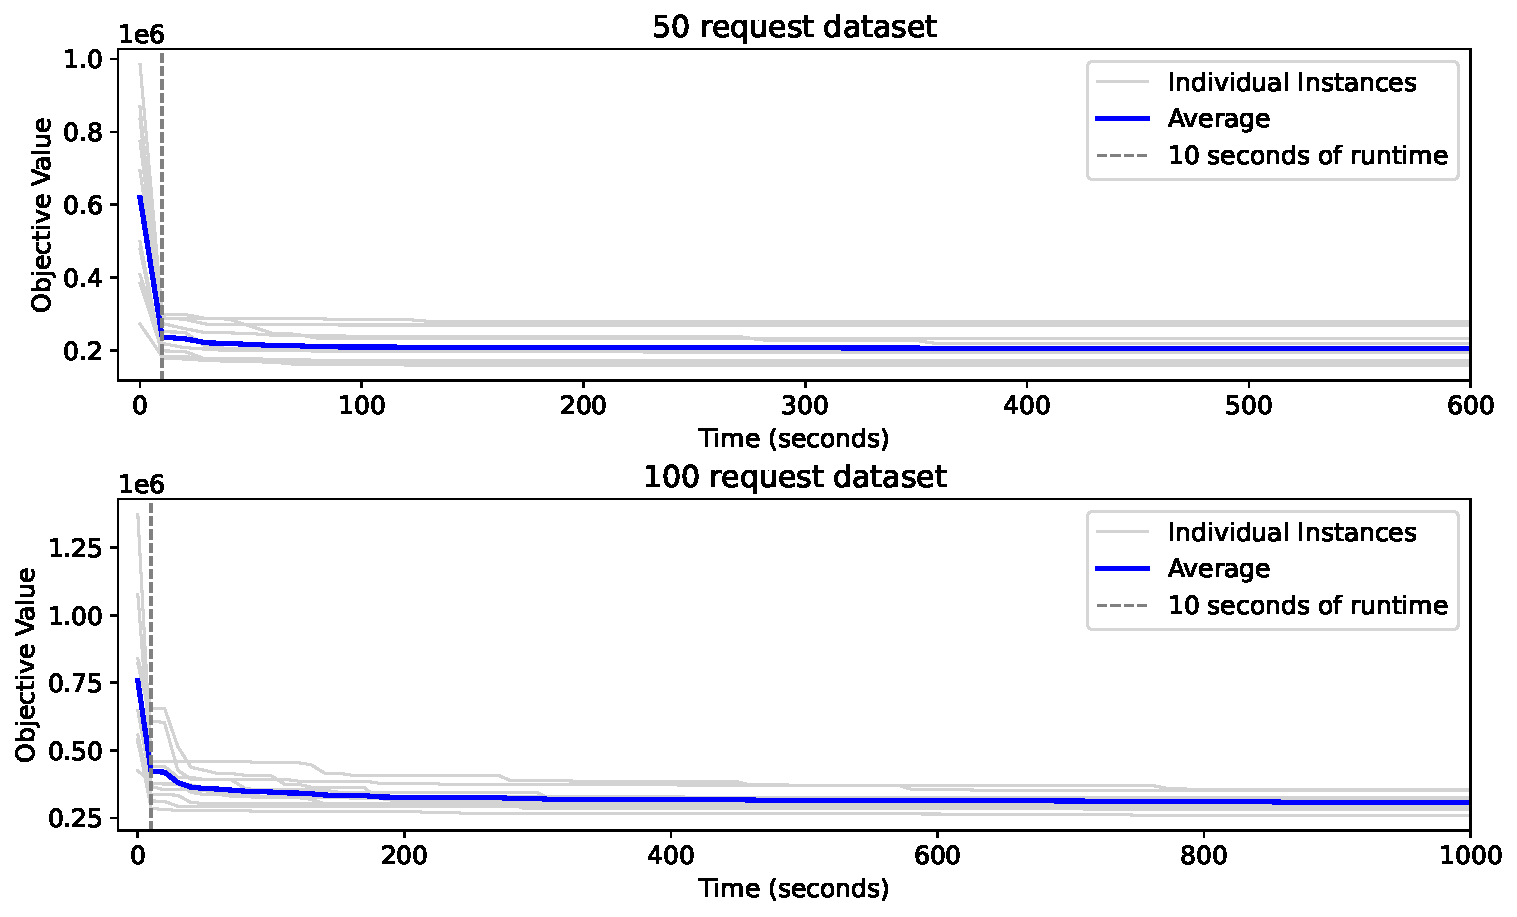
\includegraphics[width=\textwidth]{figures/graph-times.pdf}
        \caption{The evolution of the objective value through running time on 50 and 100 request datasets.}
        \label{fig:graph-times}
    \end{figure}

    \begin{figure}[!ht]
        \centering
        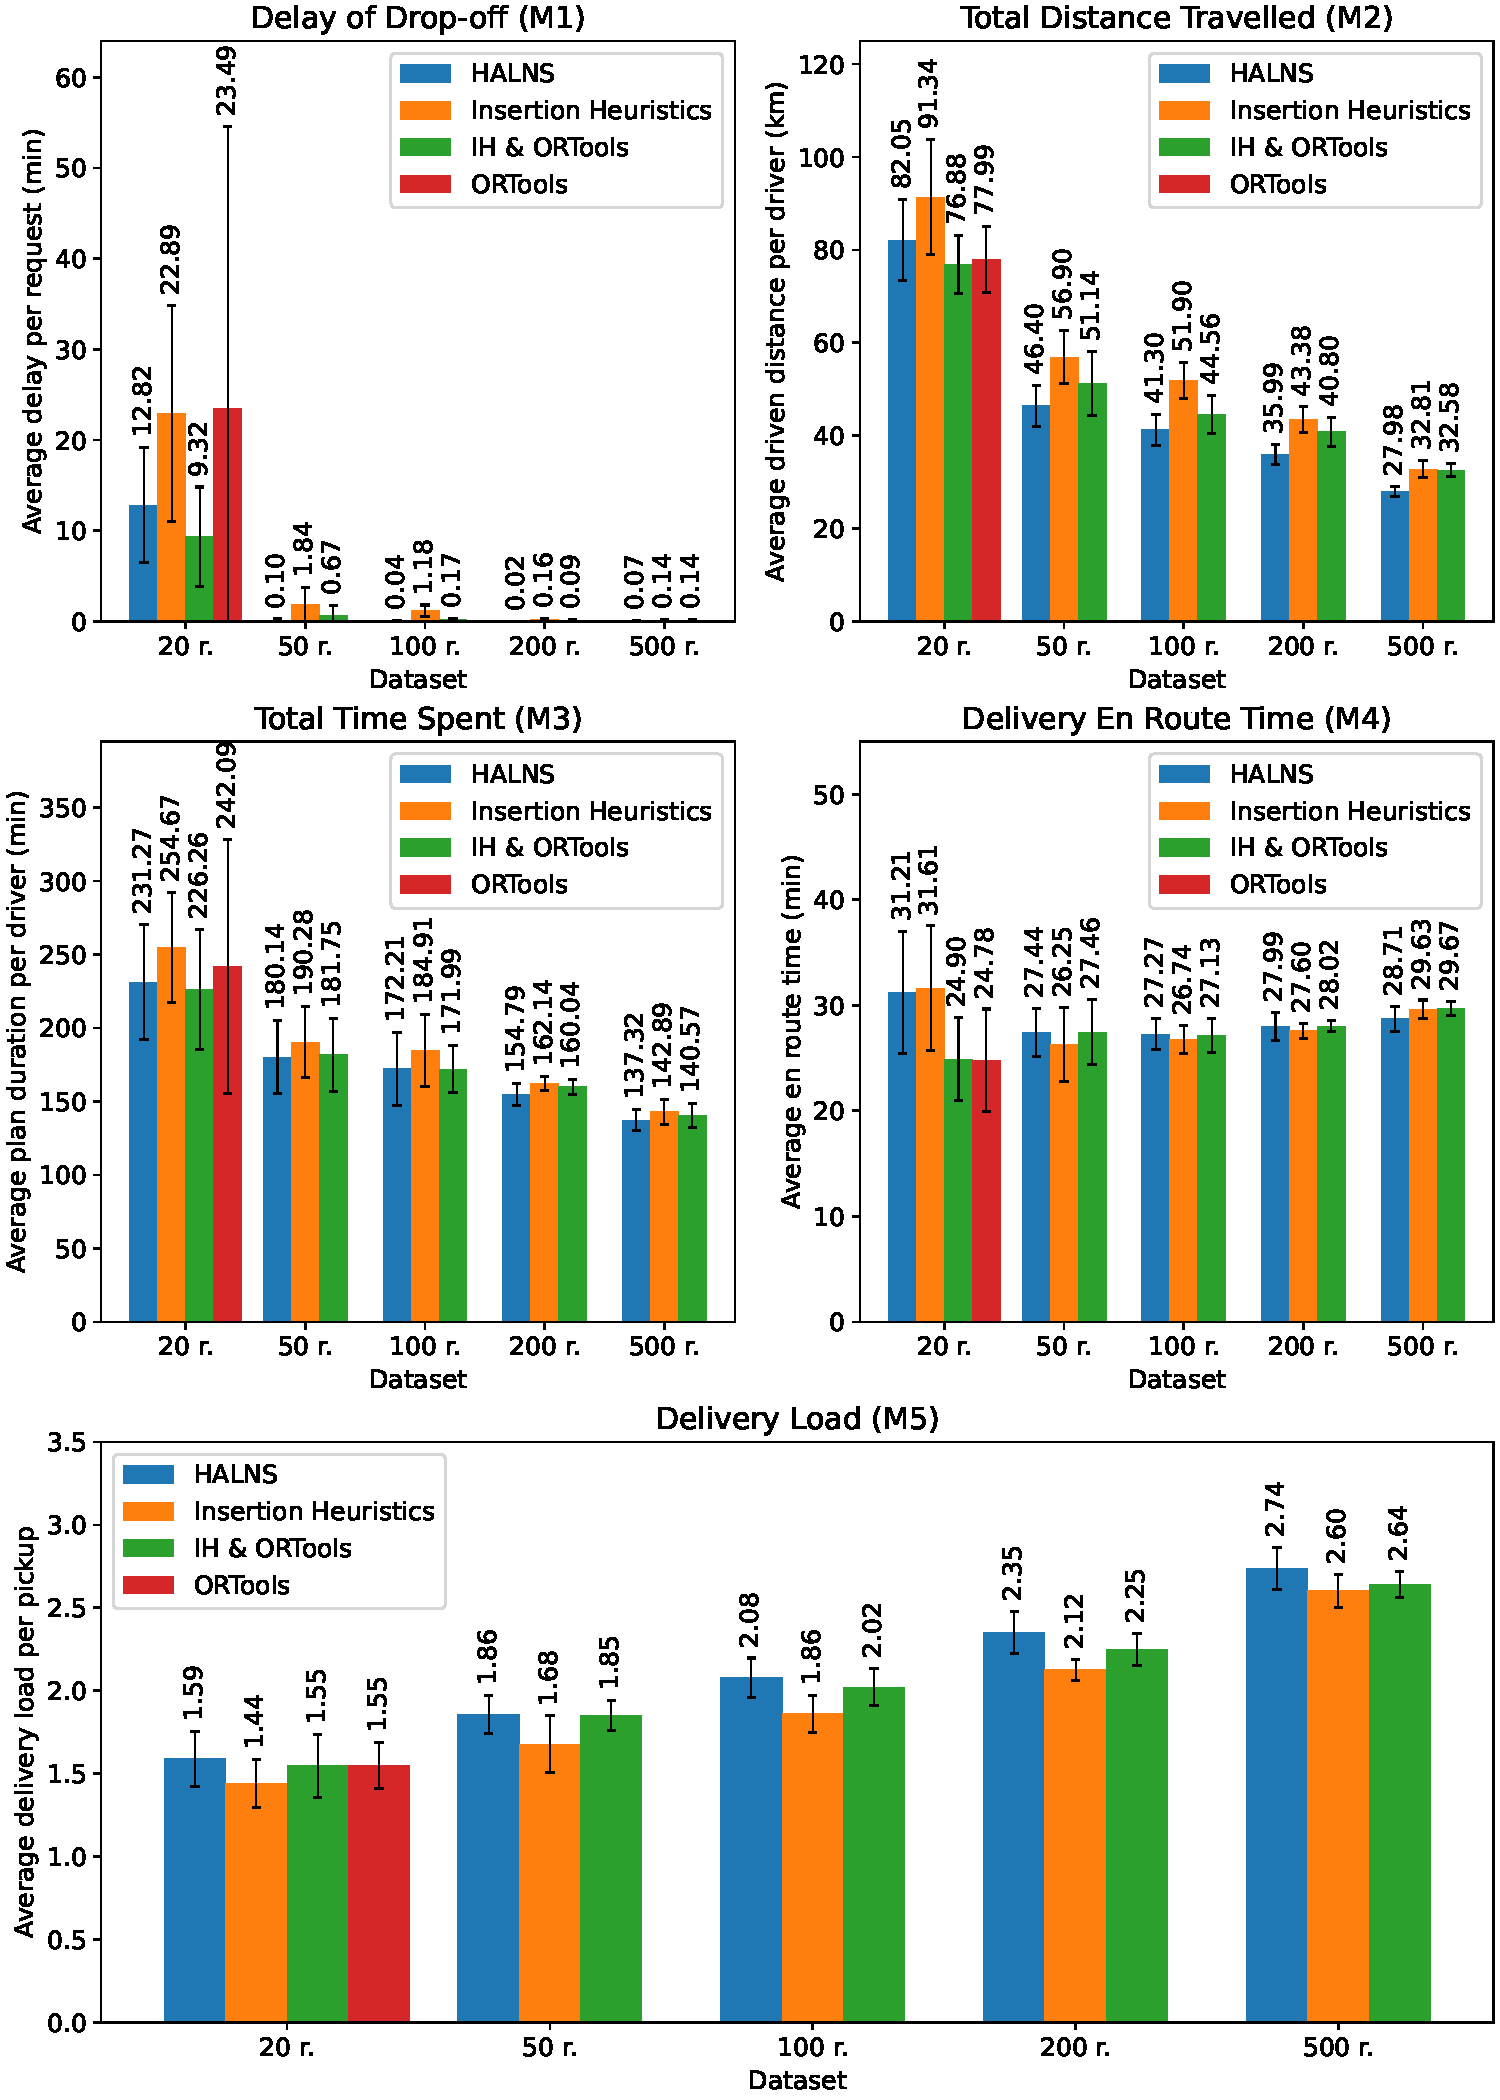
\includegraphics[width=\textwidth]{figures/metrics-graphs.pdf}
        \caption{Results of metrics M1 - M5 evaluated on our 5 datasets, averaged from 10 runs of each instance in each dataset.}
        \label{fig:metrics-graphs}
    \end{figure}
    
    
    The objective is to minimize the total delay and the total distance by using the formula $cost(e) = \beta t^{\mathrm{delay}}_e + \gamma t^{\mathrm{distance}}_e$ for each route $e$ with the parameters $\beta = 1$ and $\gamma = 0.5$, as detailed in sections \ref{halns:cost} and \ref{halns:parameters}. Therefore, we observe the tradeoff between the total delay accumulated on all requests in the instance and the total distance travelled by all drivers. The figure \ref{fig:graph-tradeoff} shows this tradeoff for each solution in our datasets. The figure \ref{fig:graph-tradeoff} confirms that the HALNS algorithm produces the overall best solutions without any outliers, compared to the baseline methods.
    
    \begin{figure}[!ht]
        \centering
        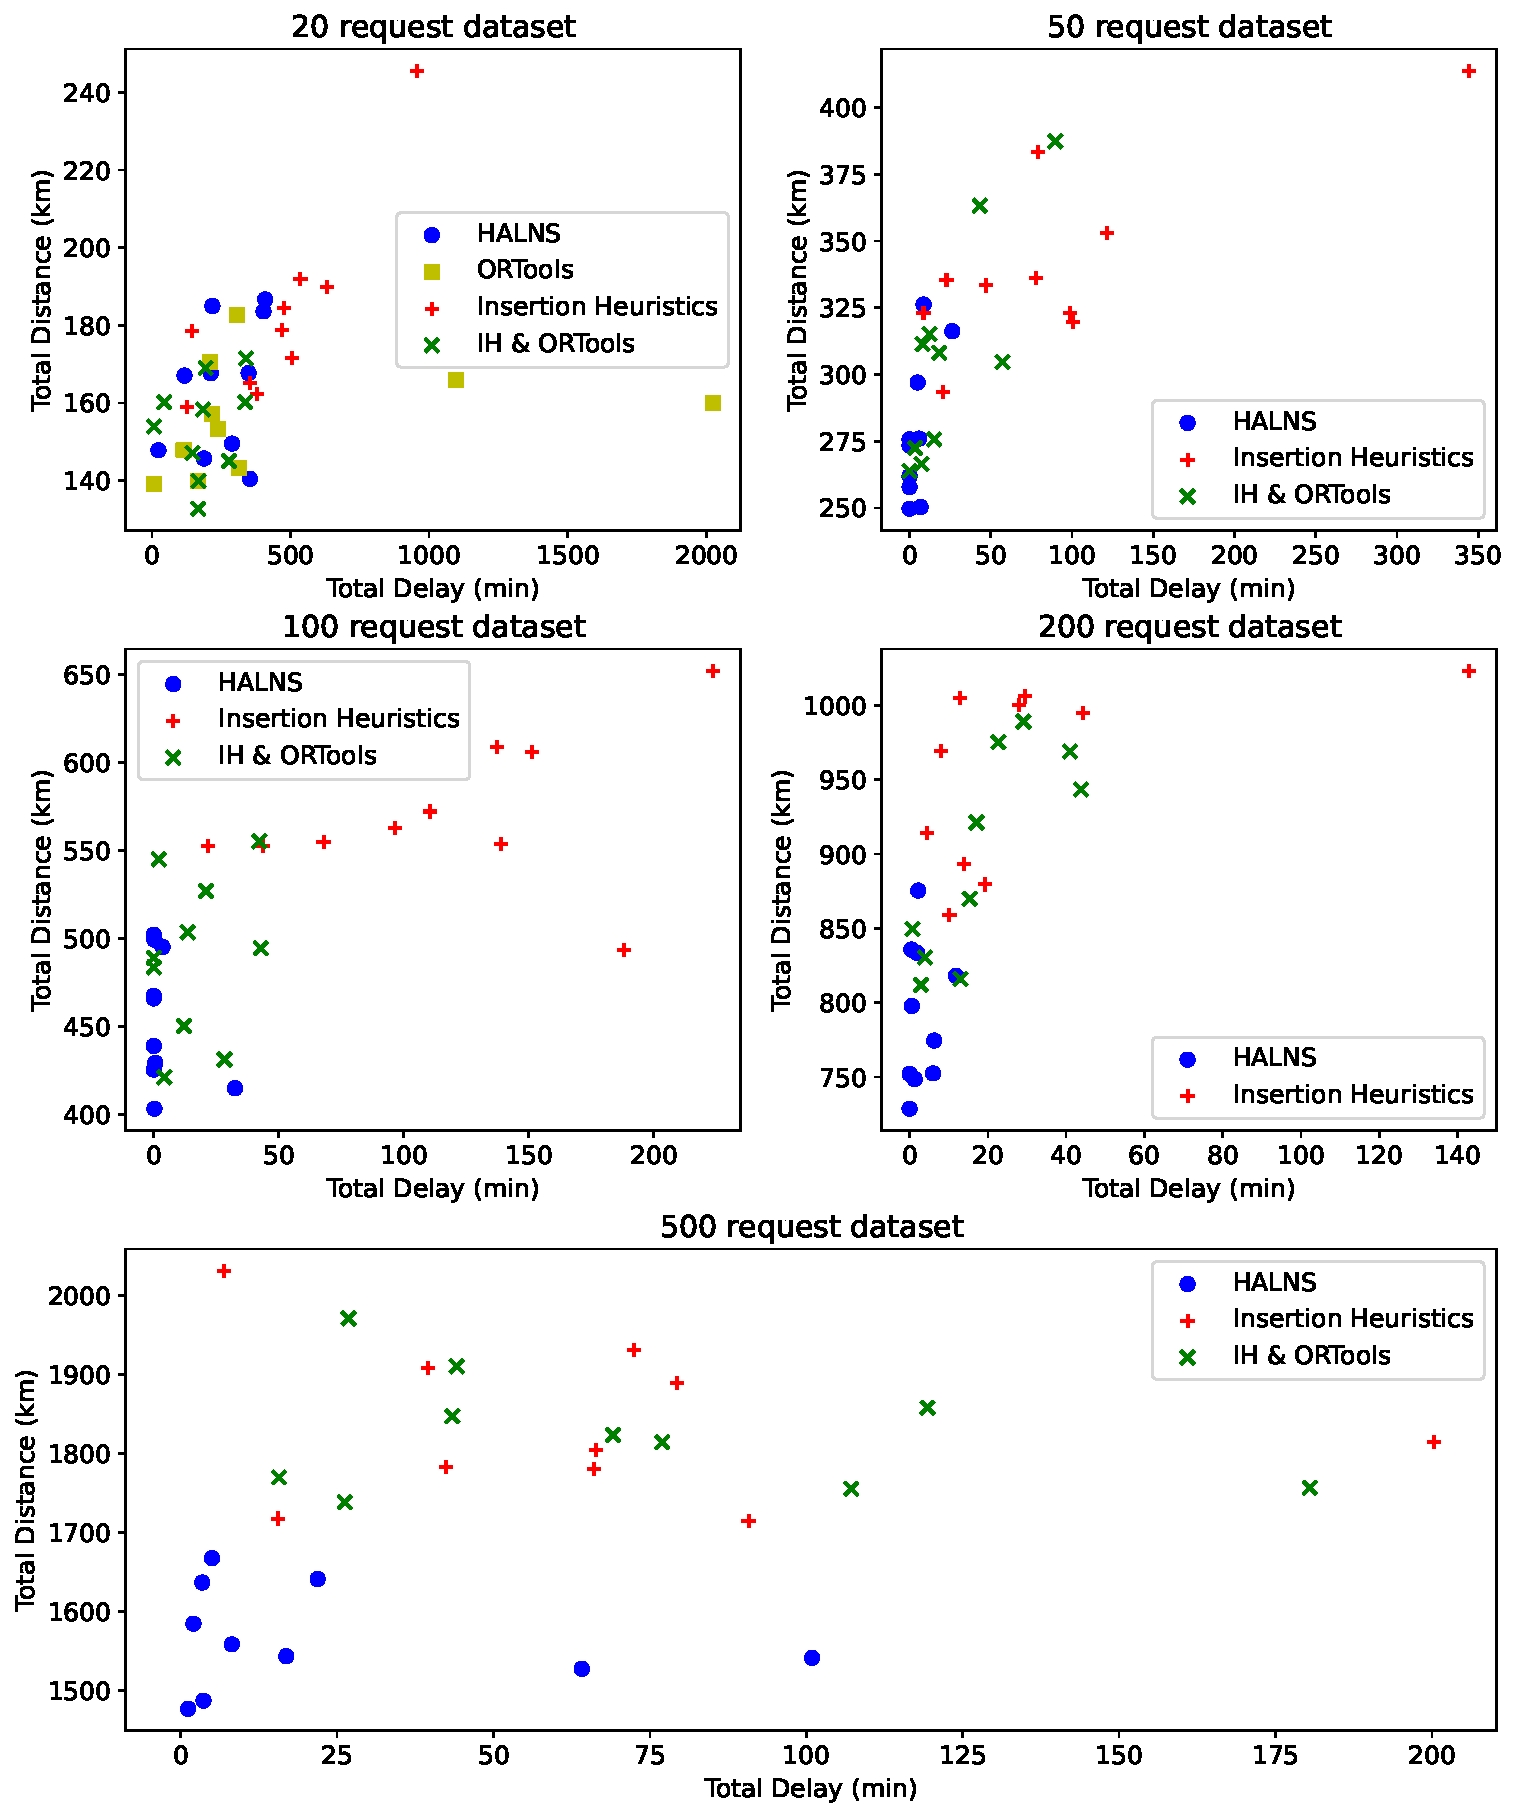
\includegraphics[width=0.9\textwidth]{figures/graph-tradeoff-2.pdf}
        \caption{The tradeoff between the total delay and the total distance for each solution produced by the individual algorithms.}
        \label{fig:graph-tradeoff}
    \end{figure}
    

    
    
    \section{Experiments on Adaptive Weight Adjustment}
    
    This section provides some results regarding the adaptive weight adjustment procedure and details the selection process of parameters $\pi_1$, $\pi_2$ and $\pi_3$ that are used to update the weights of the operators based on their past performance, as thoroughly described in section \ref{halns:weight}.
    
    To select the parameters $\pi_1$, $\pi_2$ and $\pi_3$ we conducted an experiment with different combinations of these parameters and compared the results. This experiment was run on a single dataset of 50 requests. It was executed 10 times and the results were averaged. The possible combinations are based on the study by Masmoudi et al. (2016) \cite{Masmoudi2016}. The produced solutions are in this case compared only by the objective function as only the HALNS algorithm is employed in this experiment. The results are shown in table \ref{tab:parameter-experiments}.
    
    Based on these results, the combination of parameters that works the best for this dataset is $(\pi_1, \pi_2, \pi_3) = (15, 5, 10)$, which was also used by Masmoudi et al. (2020) \cite{Masmoudi2020} and which follows the proposal of Ropke et al. (2006) \cite{Ropke2006} that $\pi_1 > \pi_3 > \pi_2$ to reinforce the diversification and thus escaping the local minima. All experiments were conducted with this set of parameters.
    
    \afterpage{
    \clearpage
    \thispagestyle{empty}
    \begin{landscape}
        \centering
        {\renewcommand{\arraystretch}{1.5}
    \begin{tabular}{llllllllll}
    \hline
    \textbf{Instance} & \multicolumn{9}{l}{\textbf{Parameters ($\pi_1$, $\pi_2$, $\pi_3$)}}                                                       		 \\ \hline
    \textbf{}         & (15, 5, 10)         &  (1, 10, 5)        &  (1, 5, 10)        &  (1, 5, 5)         &  (10, 1, 5)    &  (10, 5, 1) &  (15, 10, 5) &  (1, 1, 1) &  (5, 1, 5)        \\ \hline
    1                 & 195077   &    197960   &    195018   &   197029   &    \textbf{194462}   &    195633   &     195356   &     198399   &   195077          \\
    2                 & \textbf{214410}   &    227528   &    219882   &   219768   &    219882   &    \textbf{214410}   &     221973   &     243910   &   220435          \\
    3                 & 197892   &    196654   &    196654   &   197996   &    \textbf{196016}   &    196654   &     196075   &     197996   &   197892          \\
    4                 & \textbf{157259}   &    158263   &    \textbf{157259}   &   \textbf{157259}   &    158263   &    160289   &     158886   &     \textbf{157259}   &   \textbf{157259}          \\
    5                 & 270077   &    269402   &    274330   &   274741   &    274127   &    267039   &     \textbf{265941}   &     269740   &   269870          \\
    6                 & 164381   &    \textbf{161878}   &    163186   &   163802   &    164166   &    \textbf{161878}   &     163798   &     163798   &   163927          \\
    7                 & 278977   &    278977   &    287459   &   293440   &    280470   &    293440   &     293440   &     \textbf{277466}   &   287602          \\
    8                 & 210639   &    231503   &    213496   &   \textbf{205610}   &    235613   &    206667   &     236569   &     210842   &   214837          \\
    9                 & 172892   &    173621   &    \textbf{170469}   &   172849   &    172849   &    173098   &     173621   &     173897   &   173144          \\
    10                & 170499   &    173052   &    169367   &   \textbf{169296}   &    169870   &    171091   &     170308   &     170745   &   \textbf{169296}          \\ \hline
    \textbf{Average}  & \textbf{203210.3} &    206883.8 &    204712.0 &   205179.0 &    206571.8 &    204019.9 &     207596.7 &     206405.2 &   204933.9
    \end{tabular}}
    \captionof{table}{Quality of produced solutions on instances of 50 requests with different combinations of parameters $\pi_1$, $\pi_2$ and $\pi_3$. Values in bold represent the minima.}
    \label{tab:parameter-experiments}
    \end{landscape}
    \clearpage
    }

    
    The performance of four insertion operators and five removal operators were studied. Figures \ref{fig:graph-insertion} and \ref{fig:graph-removal} show how the weights of the operators are updated in the first 3000 iterations of the search on a single, randomly selected instance. Similarly, tables \ref{tab:res-operator-percentage-insertion} and \ref{tab:res-operator-percentage-removal} in the appendix \ref{app:tables} show the percentage of time each insertion and removal operators were used within 5 minutes of runtime on all instances of the 100 request dataset, averaged from 10 runs of each. The results in table \ref{tab:res-operator-percentage-removal} show that the removal operators have comparable frequencies of usage. The reason behind that may be the fact that in most cases two removal operators are applied. In contrast, the insertion operators are much more imbalanced. The operators I2 and I4 are used much more often than the other two, probably because these two operators are greedier in terms of finding the best insertion point across all routes rather than in a single route.
    
    \begin{figure}[!ht]
        \centering
        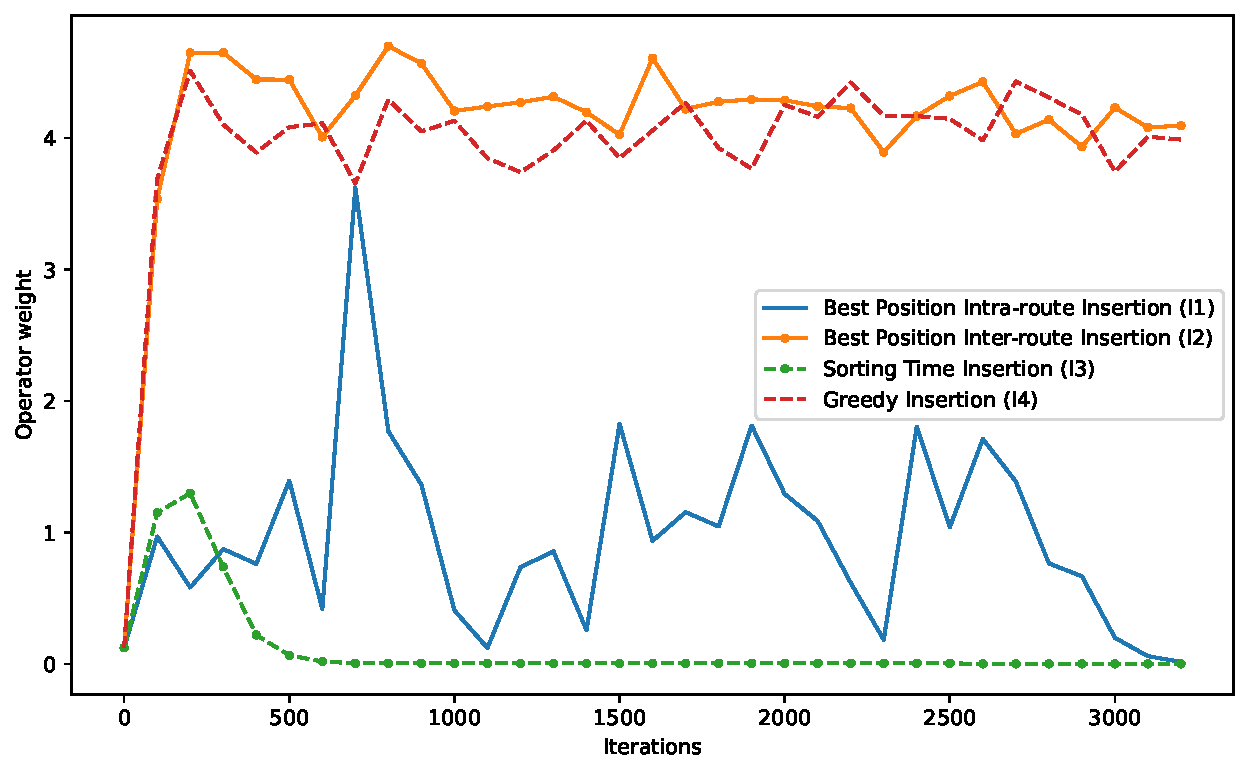
\includegraphics[width=0.9\textwidth]{figures/insertion-operators.pdf}
        \caption{Update of the weights of our four insertion operators during the first 3\,000 iterations on a single instance.}
        \label{fig:graph-insertion}
    \end{figure}
    
    \begin{figure}[!ht]
        \centering
        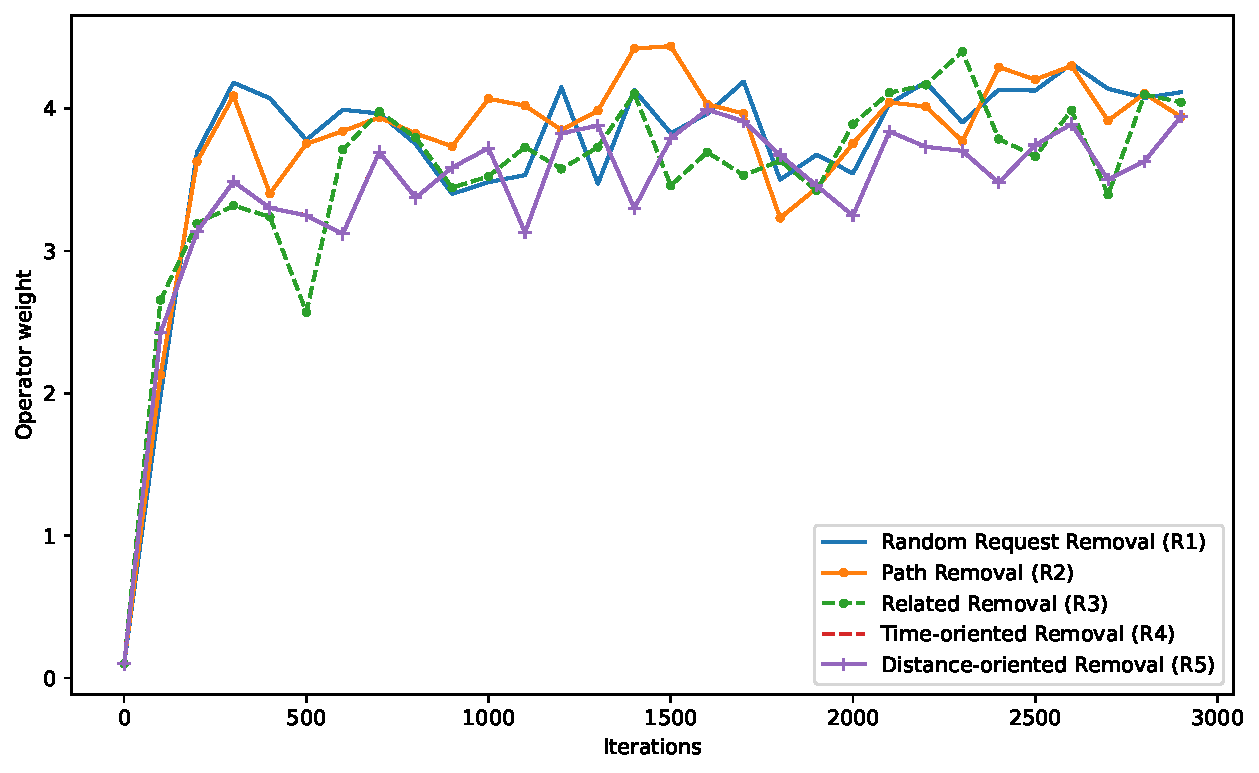
\includegraphics[width=0.9\textwidth]{figures/removal-operators.pdf}
        \caption{Update of the weights of our five removal operators during the first 3\,000 iterations on a single instance.}
        \label{fig:graph-removal}
    \end{figure}

    
    
    We also studied the complexity of the insertion and removal operators using the Go profiler. Table \ref{tab:operators-cpu} shows the CPU time used by each operator within 5 minutes of runtime. As expected, the greedy insertion operator I4 takes the most CPU time.


\setsecnumdepth{part}
\chapter{Conclusion} \label{chapter:conclusion}
With the evergrowing popularity of delivery services, customers do no longer settle for a mediocre experience. This is especially true in the food delivery market, where customers demand the fastest possible delivery time for the lowest possible cost. To be able to compete in this market, companies depend upon efficient planning and order dispatching, which has to be done in real time given the dynamic environment of gastronomy.

This study contributes to the area of vehicle routing problems. We have devised a method to solve the PDPTW in the food delivery settings that uses several novel approaches adopted from the recent studies. The usefulness of our work lies in the integration of the planning algorithm to the GoDeliver system and its successful deployment to the real customers.

The proposed algorithm is adopted mainly from the research of DARP by Masmoudi et al. (2020) \cite{Masmoudi2020} and adapted to the PDPTW by introducing different constraints and objectives, as well as altered operators and custom parameters. The algorithm was implemented in Go language and benchmarked against insertion heuristics and Google's ORTools.

We have obtained encouraging results demonstrating that the proposed algorithm is able to solve large-scale instances emanating from real-life usecases. The results also emphasize the importance of the combination of intensification and diversification mechanisms within the search.

An important issue to address in future is regarding the performance of the algorithm. Additional performance optimization and parallelization is needed to achieve faster and more predictable execution times, which would make it easier to scale the algorithm to even larger instances. Moreover, further parameter tuning could help to find overall better solutions.


\bibliographystyle{iso690}
\bibliography{resources}

\setsecnumdepth{all}
\appendix

\chapter{Acronyms}
\begin{description}
	
	\item[ALNS] Adaptive Large Neighborhood Search
	\item[API] Application Programming Interface
	\item[ARP] Arc Routing Problem
	\item[B\&B] Branch-and-Bound
	\item[CVRP] Capacitated Vehicle Routing Problem
	\item[DAFP] Dial-a-Flight Problem
	\item[DARP] Dial-a-Ride Problem
	\item[FSMVRP] Fleet Size and Mix Vehicle Routing Problem
	\item[HALNS] Hybrid Adaptive Large Neighborhood Search
	\item[HFVRP] Heterogenous Fleet Vehicle Routing Problem
	\item[HFVRPTW] Heterogenous Fleet Vehicle Routing Problem with Time Windows
	\item[HVRP] Heterogenous Vehicle Routing Problem
	\item[PDP] Pickup and Delivery Problem
	\item[PDPTW] Vehicle Routing Problem with Time Windows
	\item[TSP] Travelling Salesman Problem
	\item[VROOM] Vehicle Routing Open-source Optimization Machine
	\item[VRP] Vehicle Routing Problem
	\item[VRPPD] Vehicle Routing Problem with Pickup and Delivery
	\item[VRPTW] Vehicle Routing Problem with Time Windows

\end{description}


\chapter{Contents of an enclosed CD}

Also available via \url{https://github.com/davidmokos/halns}.

\begin{figure}
	\dirtree{%
    	.1 README.md\DTcomment{the file with the instructions}.
        .1 godeliver-planner\DTcomment{the folder with the GoDeliver Planner service}.
		.1 halns\DTcomment{the HALNS implementation in Go language}.
		.1 thesis\DTcomment{the directory with the thesis}.
		.2 MT\_Mokos\_David\_2021.pdf\DTcomment{the thesis text in the PDF format}.
        .2 sources\DTcomment{\LaTeX{} source codes of the thesis}.
	}
\end{figure}


\chapter{Tables} \label{app:tables}
\begin{table}[!ht]
    \centering
    {\renewcommand{\arraystretch}{1.5}
    \begin{tabular}{llllllllll}
    \hline
    \textbf{Instance} & \multicolumn{4}{l}{\textbf{Insertion Operators}}                        \\ \hline
    \textbf{}         & \textbf{I1}       & \textbf{I2}        & \textbf{I3}       & \textbf{I4}\\ \hline
    1                 & 2.23\,\%          & 46.88\,\%          & 4.32\,\%          & 46.57\,\%  \\
    2                 & 12.56\,\%         & 41.48\,\%          & 6.85\,\%          & 39.11\,\%  \\
    3                 & 11.68\,\%         & 43.46\,\%          & 2.24\,\%          & 42.61\,\%  \\
    4                 & 1.84\,\%          & 48.54\,\%          & 2.17\,\%          & 47.45\,\%  \\
    5                 & 7.24\,\%          & 46.08\,\%          & 2.29\,\%          & 44.40\,\%  \\
    6                 & 4.58\,\%          & 41.37\,\%          & 11.84\,\%         & 42.21\,\%  \\
    7                 & 3.98\,\%          & 46.53\,\%          & 1.45\,\%          & 48.04\,\%  \\
    8                 & 8.90\,\%          & 44.18\,\%          & 5.04\,\%          & 41.88\,\%  \\
    9                 & 8.13\,\%          & 42.97\,\%          & 4.54\,\%          & 44.36\,\%  \\
    10                & 4.31\,\%          & 45.59\,\%          & 6.85\,\%          & 43.24\,\%  \\ \hline
    \textbf{Average}  & \textbf{6.55\,\%} & \textbf{44.71\,\%} & \textbf{4.76\,\%} & \textbf{43.99\,\%}
    \end{tabular}}
    \caption{Percentage of use within 5 minutes of runtime of all insertion operators of HALNS algorithm.}
    \label{tab:res-operator-percentage-insertion}
    \end{table}


    \begin{table}[!ht]
    \centering
    {\renewcommand{\arraystretch}{1.5}
    \begin{tabular}{llllllllll}
    \hline
    \textbf{Instance} & \multicolumn{5}{l}{\textbf{Removal Operators}}                                                        \\ \hline
    \textbf{}         & \textbf{R1}       & \textbf{R2}        & \textbf{R3}        & \textbf{R4}        & \textbf{R5}        \\ \hline
    1                 & 22.05\,\%         & 19.48\,\%          & 19.17\,\%          & 19.73\,\%          & 19.57\,\%          \\
    2                 & 21.37\,\%         & 19.58\,\%          & 19.46\,\%          & 20.22\,\%          & 19.37\,\%          \\
    3                 & 20.36\,\%         & 19.67\,\%          & 20.47\,\%          & 20.22\,\%          & 19.28\,\%          \\
    4                 & 21.05\,\%         & 21.43\,\%          & 18.90\,\%          & 21.11\,\%          & 17.51\,\%          \\
    5                 & 20.43\,\%         & 20.80\,\%          & 19.45\,\%          & 20.86\,\%          & 18.47\,\%          \\
    6                 & 20.16\,\%         & 20.04\,\%          & 20.07\,\%          & 21.12\,\%          & 18.60\,\%          \\
    7                 & 20.43\,\%         & 21.15\,\%          & 18.56\,\%          & 20.83\,\%          & 19.04\,\%          \\
    8                 & 20.17\,\%         & 20.35\,\%          & 18.88\,\%          & 21.20\,\%          & 19.40\,\%          \\
    9                 & 22.10\,\%         & 20.00\,\%          & 19.00\,\%          & 19.97\,\%          & 18.93\,\%          \\
    10                & 20.82\,\%         & 21.44\,\%          & 19.39\,\%          & 19.48\,\%          & 18.88\,\%          \\ \hline
    \textbf{Average}  &\textbf{20.89\,\%} & \textbf{20.39\,\%} & \textbf{19.33\,\%} & \textbf{20.48\,\%} & \textbf{18.91\,\%}
    \end{tabular}}
    \caption{Percentage of use within 5 minutes of runtime of all removal operators of HALNS algorithm.}
    \label{tab:res-operator-percentage-removal}
    \end{table}
    
    \begin{table}[!ht]
    \centering
    {\renewcommand{\arraystretch}{1.5}
    \begin{tabular}{llllll}
    \hline
               & \multicolumn{5}{l}{\textbf{Insertion Operators}}                    \\
    Operator   & \textbf{I1} & \textbf{I2} & \textbf{I3} & \textbf{I4} & \textbf{}   \\ \hline
    Percentage & 2.82\,\%    & 25.33\,\%   & 2.21\,\%    & \textbf{69.64}\,\%   &             \\
    \multicolumn{6}{l}{}                                                             \\ \hline
               & \multicolumn{5}{l}{\textbf{Removal Operators}}                      \\
    Operator   & \textbf{R1} & \textbf{R2} & \textbf{R3} & \textbf{R4} & \textbf{R5} \\ \hline
    Percentage & 10.02\,\%   & 12.2\,\%    & \textbf{31.38}\,\%   & 29.98\,\%   & 16.42\,\%  
    \end{tabular}}
    \caption{Percentage of CPU used by each operator of HALNS algorithm within 5 minutes of runtime.}
    \label{tab:operators-cpu}
    \end{table}



\end{document}


